%% USPSC-Cap2-Desenvolvimento.tex 

% ---
% Este capítulo, utilizado por diferentes exemplos do abnTeX2, ilustra o uso de
% comandos do abnTeX2 e de LaTeX.
% ---

\chapter{Desenvolvimento}\label{cap-desenv}

Neste capítulo, será fornecida uma exposição ordenada e detalhada do desenvolvimento deste trabalho. Serão delineados os passos e abordagens utilizados para o treinamento e validação dos modelos, culminando na análise das variáveis mais importantes para a predição de casos de reinternação.

\section{Metodologia}\label{sec-metodologia}

A metodologia utilizada para atingir os objetivos propostos foi dividida em etapas. Inicialmente, foi feita uma definição clara do domínio do problema, seguida pela exploração do conjunto de dados. Em seguida, foram abordadas as ferramentas utilizadas, seguidas pelo processo de limpeza e preparação dos dados. Por fim, foi realizado o treinamento dos modelos e a análise das variáveis utilizando o método SHAP.

\subsection{Definiç\~ao de domínio do problema}

O problema abordado neste estudo refere-se à previsão de reinternação hospitalar de pacientes que receberam cuidados de saúde mental no sistema de informação da Coordenação de Internações em Ribeirão Preto, Brasil, no período de julho de 2012 a dezembro de 2017. Este domínio envolve a aplicação de modelos de classificação de aprendizado de máquina em um conjunto de dados específico, com o propósito de antecipar eventos de reinternação hospitalar. Além disso, o estudo incorpora técnicas de inteligência artificial explicável, notadamente o SHAP, para identificar e quantificar as variáveis que apresentam maior influência nos casos de reinternação, contribuindo assim para uma compreensão mais profunda dos fatores associados a esses eventos. A análise deste domínio visa aprimorar a capacidade de tomada de decisões e políticas de saúde, com ênfase na prevenção eficaz e na otimização dos recursos hospitalares.

\subsection{Conjunto de dados}

O conjunto de dados empregado neste estudo já foi explorado em outras pesquisas \cite{barros2016, eHealth, FeatureSensitivity}. As informações contidas neste conjunto são referentes a 8.755 pacientes, com uma média de idade de 37,6 anos. As características do conjunto de dados englobam aspectos sociodemográficos, dados sobre internações hospitalares, diagnósticos, utilização de serviços médicos, informações de alta hospitalar e registros temporais, como datas de admissão, alta ou óbito. Na \autoref{tab:dados}, são descritas quais variáveis deste conjunto foram utilizadas neste estudo.

\begin{table}
	\IBGEtab{
		\caption{\centering\label{tab:dados}Variáveis utilizadas do conjunto de dados.}
	}
	{
		\begin{tabular}{ccc}
			\toprule
			\textbf{Nome da variável} & \textbf{Tipo da variável} \\
			\midrule \midrule
   			Arranjo docimiliar & Categórica \\
   			\midrule
			AVC & Booleana \\
			\midrule
			Convulsão & Booleana \\
			\midrule
			Dia da semana na 1\textsuperscript{a} internação & Numérica (inteira) \\
			\midrule
			Diabetes & Booleana \\
			\midrule
			Diagnóstico (CID10) & Categórica \\
			\midrule
			Doença infecto & Booleana \\
			\midrule
			Estado civil & Categórica \\
			\midrule
			Etnia & Categórica \\
			\midrule
			HAS & Booleana \\
			\midrule
			Idade na 1\textsuperscript{a} internação & Numérica (inteira) \\
			\midrule
			Mês da 1\textsuperscript{a} internação & Numérica (inteira) \\
			\midrule
			Problemas respiratórios & Booleana \\
			\midrule
			Quantidade de problemas na 1\textsuperscript{a} internação & Numérico (inteira) \\
			\midrule
			Sexo & Categórica \\
			\midrule
			Situação profissão & Categórica \\
			\midrule
			Tempo de internação (em horas) & Numérica (contínua) \\
			\midrule
			Traumatismo & Booleana \\
			\bottomrule
		\end{tabular}
	}
	{
		\fonte{\centering{Autor (2023).}}
	}
\end{table}

\subsection{Ferramentas utilizadas}\label{sec:ferramentas}

Todo o desenvolvimento deste trabalho foi feito utilizando a linguagem de programação Python. Essa linguagem não apenas oferece uma sintaxe clara e concisa, mas também proporciona um vasto ecossistema de bibliotecas especializadas que simplificam e aprimoram cada etapa de um projeto de ciência de dados.

As bibliotecas Pandas e Numpy foram utilizadas na limpeza e preparação dos dados para a seleção de modelos. A escolha dessas bibliotecas deve-se à eficiência e flexibilidade que oferecem em termos de manipulação de dados, permitindo operações rápidas e simplificadas. Pandas facilita a manipulação de estruturas de dados tabulares, enquanto a Numpy fornece suporte para operações numéricas eficientes, ambos fundamentais em projetos de ciência de dados.

A biblioteca Scikit-Learn \cite{Buitinck} foi utilizada para o pré-proces\-sa\-men\-to, seleção e validação cruzada dos modelos. A escolha dessa biblioteca deve-se à sua abrangência na implementação de algoritmos de aprendizado de máquina, proporcionando uma interface consistente para a construção, avaliação e ajuste de modelos. Isso facilita a experimentação e comparação entre diferentes abordagens, agilizando o desenvolvimento do projeto.

Matplotlib e Seaborn foram as bibliotecas utilizadas na criação de visualizações em todas as etapas do projeto. A escolha dessas bibliotecas deve-se à capacidade de produzir gráficos informativos e visualmente atraentes. Isso não apenas facilita a compreensão rápida dos resultados, mas também fortalece a comunicação efetiva dos achados para diferentes públicos, desde especialistas em dados até partes interessadas não técnicas.

Por fim, a bilioteca Shap \cite{Shap2017} foi utilizada por sua capacidade de explicar as predições dos modelos de aprendizado de máquina. Isso não apenas torna as previsões mais interpretáveis, mas também fornece insights profundos sobre como cada variável contribui para as decisões do modelo, melhorando a confiabilidade e compreensão do sistema.

\subsection{Limpeza e prepação dos dados}\label{sec:limpeza}

O processo de limpeza de dados foi executado em diversas etapas para garantir a qualidade e a relevância do conjunto de dados para as análises e modelagem subsequentes. Inicialmente, foram identificadas e eliminadas variáveis redundantes para o escopo específico da tarefa em pauta, que consistia na previsão de reinternação de pacientes. Além disso, foram eliminadas variáveis que poderiam potencialmente introduzir \textit{data leakage} nos modelos a serem desenvolvidos posteriormente. Um exemplo ilustrativo desse cenário seria a presença de variáveis que forneciam informações sobre a segunda internação de um paciente. Utilizar tais informações representaria um vazamento de dados, pois indicaria ao modelo que o paciente já passou por uma reinternação, informação que não estaria disponível no momento da primeira internação. Este cuidado durante a limpeza dos dados foi essencial para preservar a integridade do processo de modelagem e garantir resultados mais precisos e confiáveis.

Dado que a natureza dos dados envolve preenchimentos manuais, tornou-se essencial padronizar e simplificar as categorias para garantir consistência e facilitar a interpretação. Variáveis como estado civil, etnia e arranjo domiciliar foram submetidas a procedimentos específicos para aprimorar a qualidade das informações. O arranjo domiciliar, por exemplo, representado por uma variedade de termos como \q{sozinho}, \q{com companheiro(a)}, \q{com filhos(as)}, entre outros, foi tratado por uma função que simplificou as categorias, mapeando-as para as opções mais abrangentes como \q{acompanhado} ou \q{sozinho}. Esse tipo de simplificação não apenas facilitou a análise, mas também reduziu a complexidade do conjunto de dados.

As variáves relacionadas a data (data de internação, data de alta e data de nascimento) foram tratadas e serviram de base para a criação de novas variáveis que buscam aprimorar a compreensão do comportamento dos pacientes e, consequentemente, melhorar as previsões dos modelos. Por exemplo, a variável \q{\textbf{mes\_data\_internacao}} indica o mês da internação, enquanto \q{\textbf{dia\_semana\_data\_internacao}} representa o dia da semana. Esses atributos têm o potencial de capturar padrões sazonais ou comportamentais que podem influenciar as chances de reinternação. Além disso, a idade do paciente na data da internação foi calculada para investigar se ela tem algum impacto nas taxas de reinternação. Uma métrica de tempo, \q{\textbf{tempo\_internacao\_horas}}, foi introduzida para avaliar a duração da internação em horas, proporcionando uma perspectiva mais granular do tempo de permanência. Essas novas variáveis foram concebidas com a intenção de enriquecer o conjunto de dados e investigar se fatores temporais específicos estão relacionados à probabilidade de reinternação.

Como o conjunto de dados trata de informações coletadas na internação, ele não tem por definição uma variável que pode ser usada como variável alvo para reinternação, portanto, ela precisou ser criada. Para estabelecer a variável-alvo \q{reinternacao}, foi desenvolvido um procedimento que utiliza a contagem de ocorrências de cada paciente para determinar se houve reinternação, considerando como critério a presença de mais de uma internação para um mesmo paciente. Além disso, um outro procedimento foi aplicado para extrair as informações exclusivas da primeira internação de cada paciente. Essa estratégia não apenas evita o vazamento de dados, mas também contribui para a integridade da modelagem, garantindo que as previsões sejam baseadas unicamente nas informações disponíveis até o momento da primeira internação. Na \autoref{img:criarTarget}, é ilustrado um exemplo do funcionamento desses procedimentos e quais dados são considerados no conjunto final.

\begin{figure}
	\centering
	\caption{\label{img:criarTarget}Fluxograma ilustrando o processo de criação da variável-alvo \q{reinternação} e a filtragem para extrair informações da primeira internação de cada paciente. Na parte superior, o estado inicial do conjunto de dados com múltiplas internações. Na parte inferior, o conjunto final, otimizado para as próximas fases de pré-processamento e treinamento dos modelos, após a aplicação das funções.}
	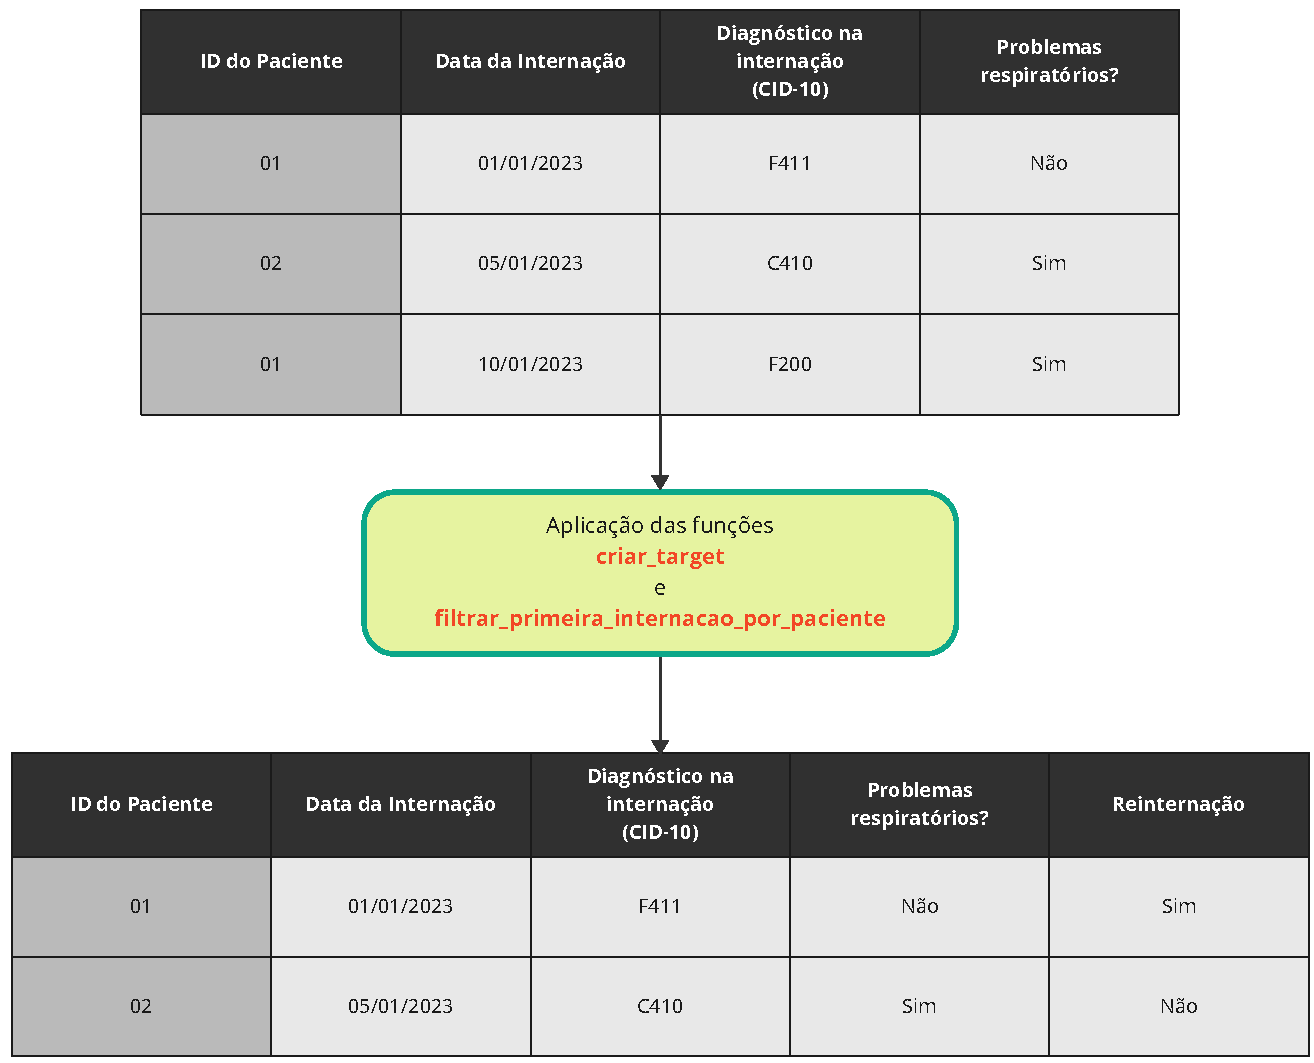
\includegraphics[scale=0.7]{USPSC-img/criacao_target.pdf}
	\begin{center}
		Fonte: Autor (2023).
	\end{center}
\end{figure}

Em resumo, a fase de limpeza e preparação dos dados foi meticulosa, visando a qualidade e relevância necessárias para análises e modelagem. Redundâncias e potenciais fontes de vazamento foram eliminadas, garantindo a integridade do processo de modelagem. A padronização de categorias simplificou a interpretação e a manipulação cuidadosa de variáveis relacionadas a datas introduziu novas características, buscando capturar padrões temporais relevantes para a previsão de reinternação. Na \autoref{img:fluxoLimpeza}, é apresentado um fluxograma visualizando todas as transformações aplicadas ao conjunto inicial de dados, delineando as etapas que culminaram no conjunto final, pronto para as próximas fases de pré-processamento e treinamento dos modelos.

\begin{figure}
	\centering
	\caption{\label{img:fluxoLimpeza}Fluxograma representando as transformações aplicadas ao conjunto inicial de dados durante o processo de limpeza e preparação.}
	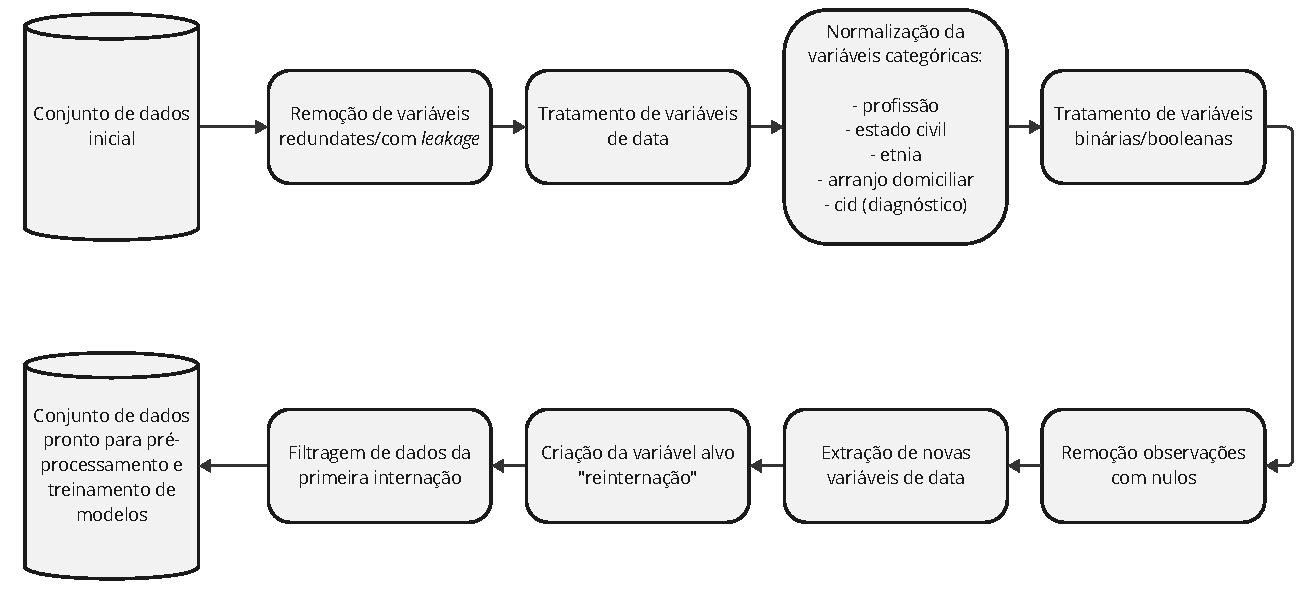
\includegraphics[scale=0.7]{USPSC-img/fluxo-limpeza.pdf}
	\begin{center}
		Fonte: Autor (2023).
	\end{center}
\end{figure}

\subsection{Treinamento dos classificadores}

A fase de treinamento e seleção dos classificadores tem início com a subdivisão do conjunto de dados em conjuntos distintos para treinamento e teste (o conjunto de teste foi empregado exclusivamente para validar os modelos já treinados, e nunca para a calibração destes modelos). Em seguida, utilizando as interfaces \textit{BaseEstimator} e \textit{TransformerMixin} do Scikit-Learn \cite{Buitinck}, foi definido um \textit{Transformer} que foi especialmente projetado para lidar com variáveis de data. Sua funcionalidade é de converter uma única coluna de datas em duas novas, aplicando as funções trigonométricas seno e cosseno sobre os valores originais da data. Essa abordagem traz uma vantagem, pois captura o padrão cíclico inerente às datas. Por exemplo, ao considerar o mês do ano em uma escala de 1 a 12, a distância entre os meses 12 e 1 é intuitivamente curta, representando uma transição direta de dezembro para janeiro. No entanto, essa distância não é adequadamente expressa por uma simples diferença aritmética de 11 unidades. As transformações seno e cosseno, ao incorporar a posição angular da data no ciclo anual, são capazes de preservar essa relação cíclica de maneira mais precisa.

As variáveis numéricas foram padronizadas, enquanto as categóricas foram tratadas por meio de codificação \textit{one-hot}. Adicionalmente, para equilibrar a variável resposta, foi aplicado undersampling, reduzindo a predominância da classe majoritária. Na \autoref{img:preProcessamento}, é apresentado o \textit{pipeline} completo de pré-processamento de dados.

\begin{figure}[H]
	\centering
	\caption{\label{img:preProcessamento}\textit{Pipeline} de pré-processamento dos dados.}
	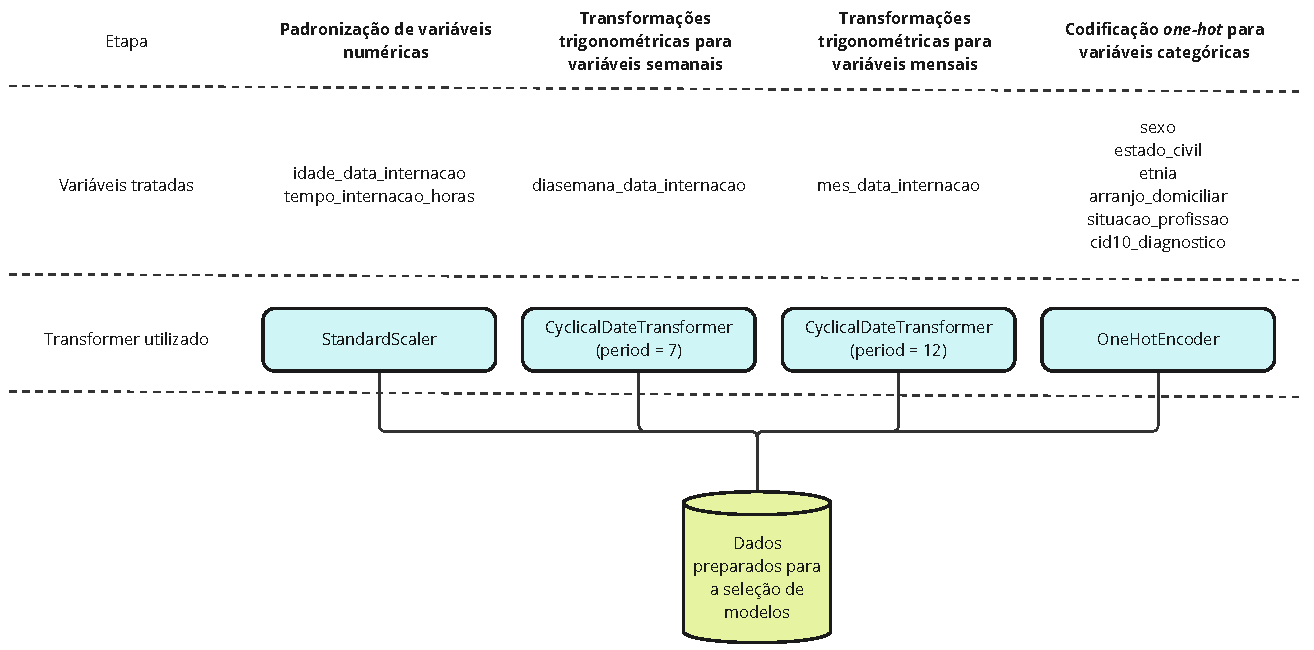
\includegraphics[scale=0.7]{USPSC-img/preprocessamento.pdf}
	\begin{center}
		Fonte: Autor (2023).
	\end{center}
\end{figure}

\subsubsection{Treinamento sem otimização de hiperparâmetros}\label{sec:treinoSemHiperparametros}

A etapa inicial do treinamento dos modelos foi conduzida sem a otimização de hiperparâmetros. A estratégia adotada envolveu a aplicação de sete algoritmos de aprendizado de máquina, com o objetivo de avaliar o desempenho inicial de cada modelo antes de otimizar seus hiperparâmetros.

Inicialmente, foi desenvolvido um \textit{Pipeline} que abrangeu os dois estágios necessários: o pré-processamento dos dados e o ajuste do modelo. A avaliação do desempenho dos modelos ocorreu por meio de validação cruzada estratificada com cinco \textit{folds} (\textit{Stratified K-Fold Cross-Validation}). Métricas fundamentais para a tarefa de classificação binária foram empregadas, abrangendo acurácia, precisão, \textit{recall} e a área sob a curva ROC (AUC-ROC).

É relevante ressaltar a importância de cada uma dessas métricas para esse tipo de análise, que visa prever reinternações de pacientes. A acurácia reflete a precisão global do modelo, enquanto a precisão destaca a proporção de instâncias positivas corretamente classificadas. O \textit{recall}, por sua vez, destaca a habilidade do modelo em capturar a totalidade das instâncias positivas, sendo crucial quando o foco está na minimização de falsos negativos, ou seja, quando é crucial identificar todos os casos de reinternação. Já a área sob a curva ROC proporciona uma métrica abrangente da capacidade discriminativa do modelo em diferentes limiares de probabilidade, sendo particularmente útil em tarefas de classificação desbalanceada \cite{geron2022hands}.

Cada modelo foi treinado e avaliado em cada uma das cinco partições do conjunto de treinamento. Na \autoref{img:curvasRocSemTunagem}, são apresentadas as curvas ROC e os valores da área para cada um dos \textit{folds}.

\begin{figure}
	\centering
	\caption{\label{img:curvasRocSemTunagem}Curvas ROC para cada um dos classificadores e cada \textit{fold} da validação cruzada.}
	
	\begin{minipage}[t]{0.28\textwidth}
		\centering
		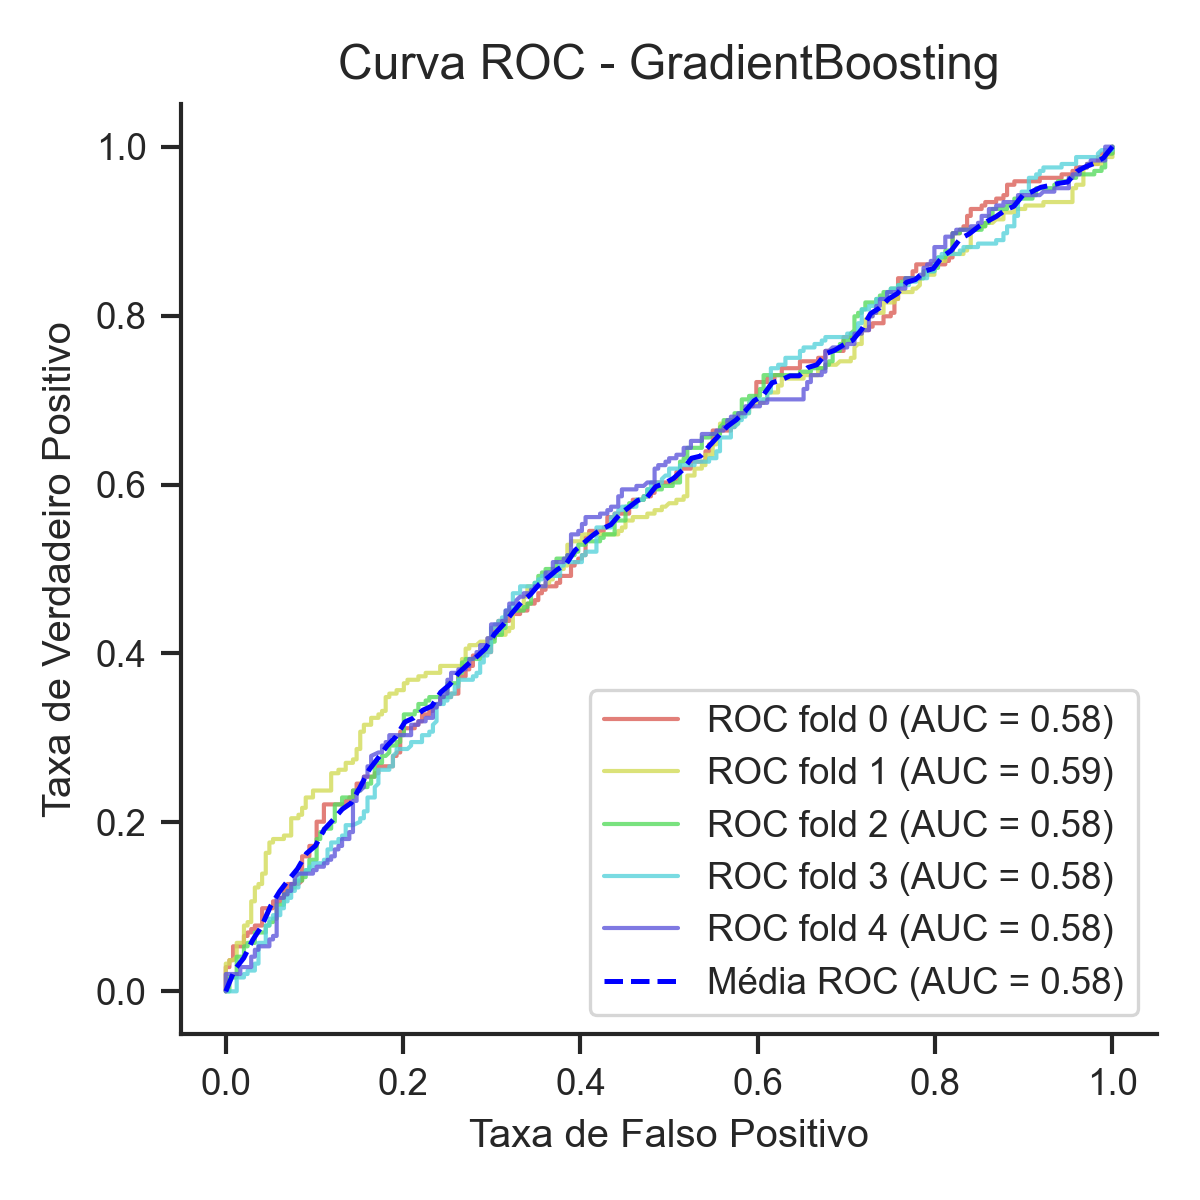
\includegraphics[width=\textwidth]{USPSC-img/Curva ROC - GradientBoosting.png}
	\end{minipage}
	\hfill
	\begin{minipage}[t]{0.28\textwidth}
		\centering
		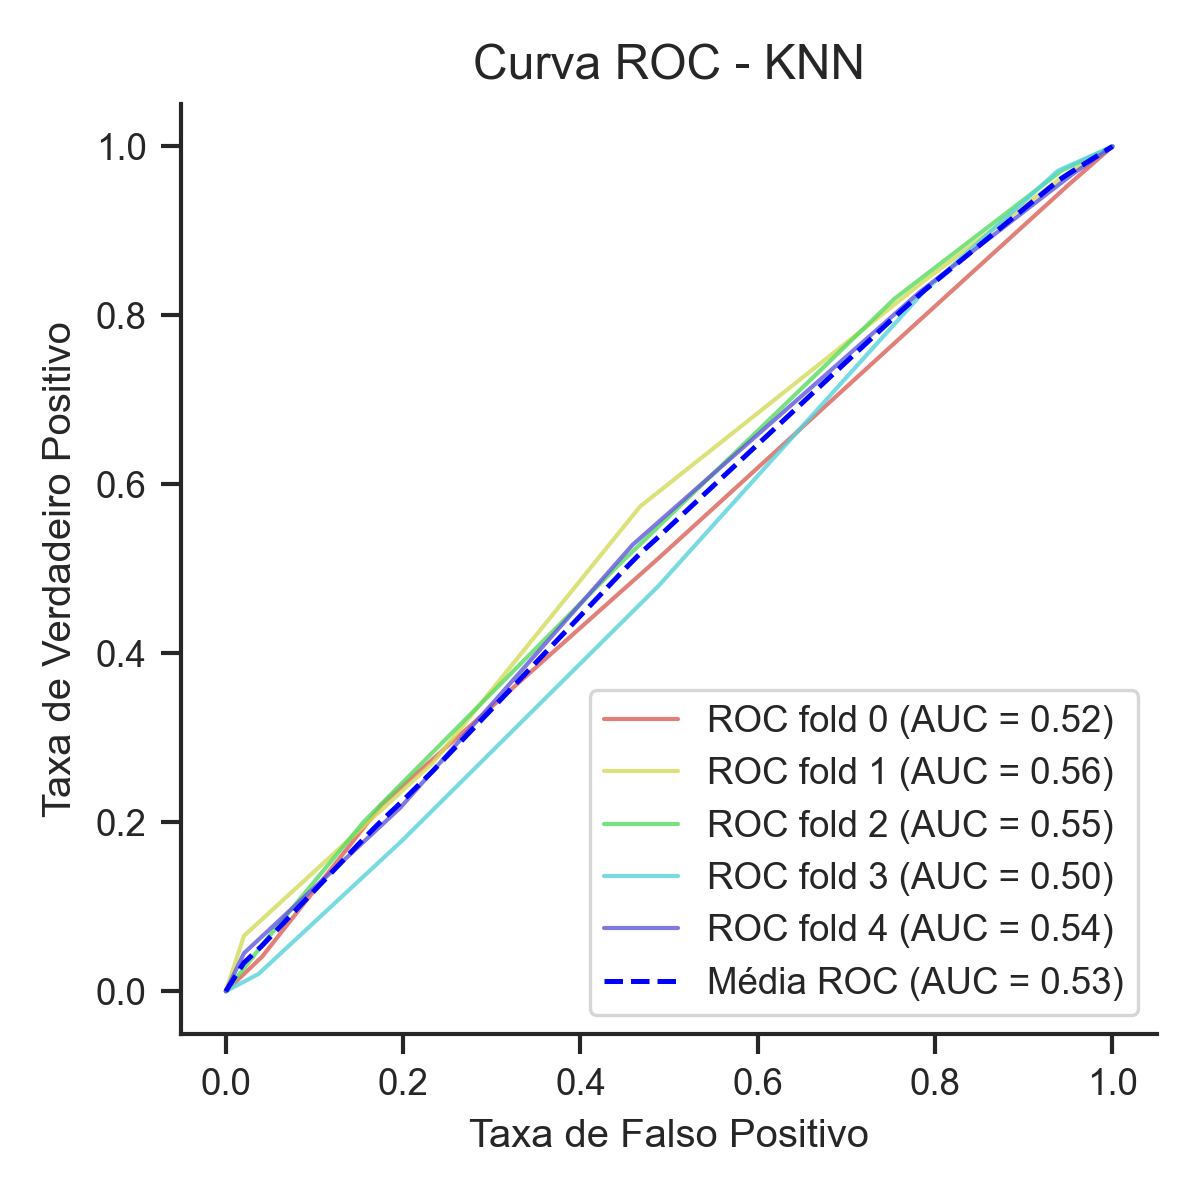
\includegraphics[width=\textwidth]{USPSC-img/Curva ROC - KNN.png}
	\end{minipage}
	\hfill
	\begin{minipage}[t]{0.28\textwidth}
		\centering
		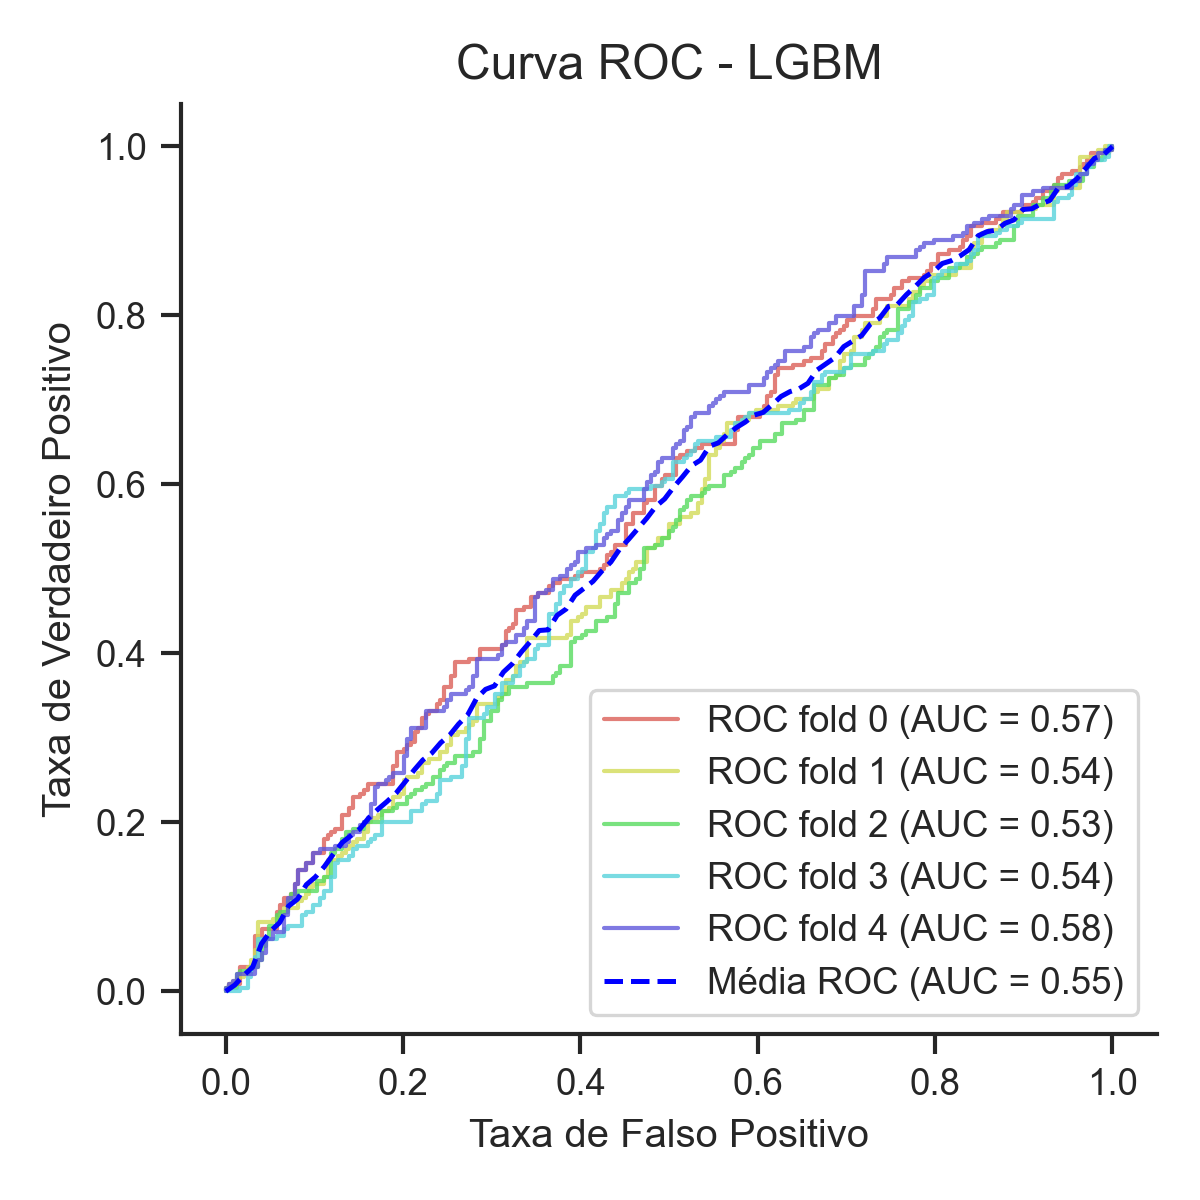
\includegraphics[width=\textwidth]{USPSC-img/Curva ROC - LGBM.png}
	\end{minipage}
	\hfill
	\begin{minipage}[t]{0.28\textwidth}
		\centering
		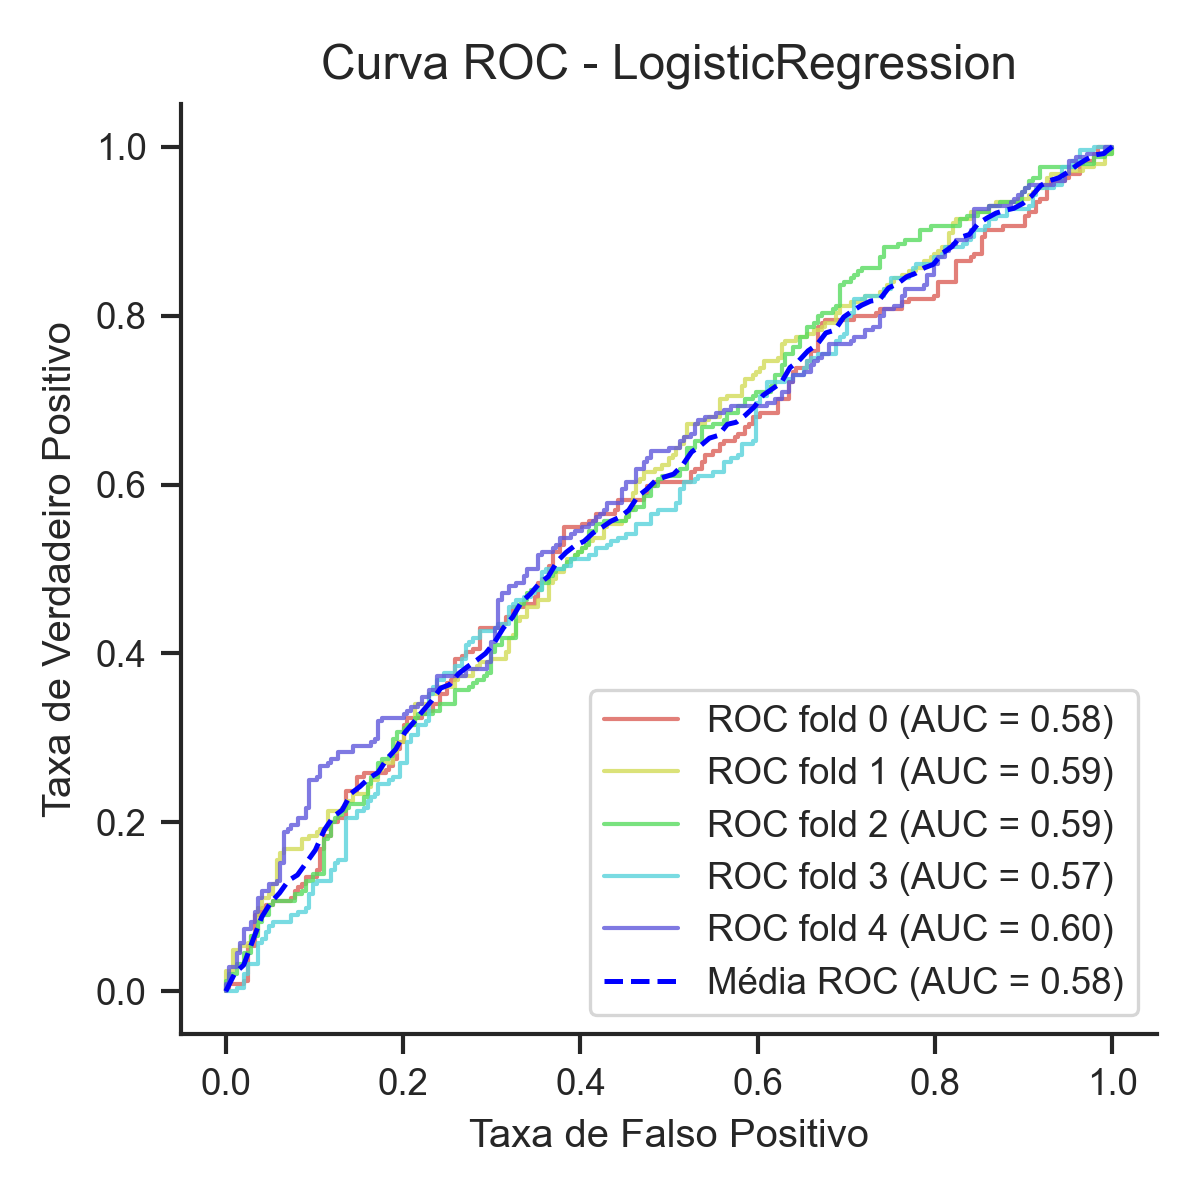
\includegraphics[width=\textwidth]{USPSC-img/Curva ROC - LogisticRegression.png}
	\end{minipage}
	
	\bigskip % Espaço vertical entre as duas filas de imagens
	
	\begin{minipage}[t]{0.28\textwidth}
		\centering
		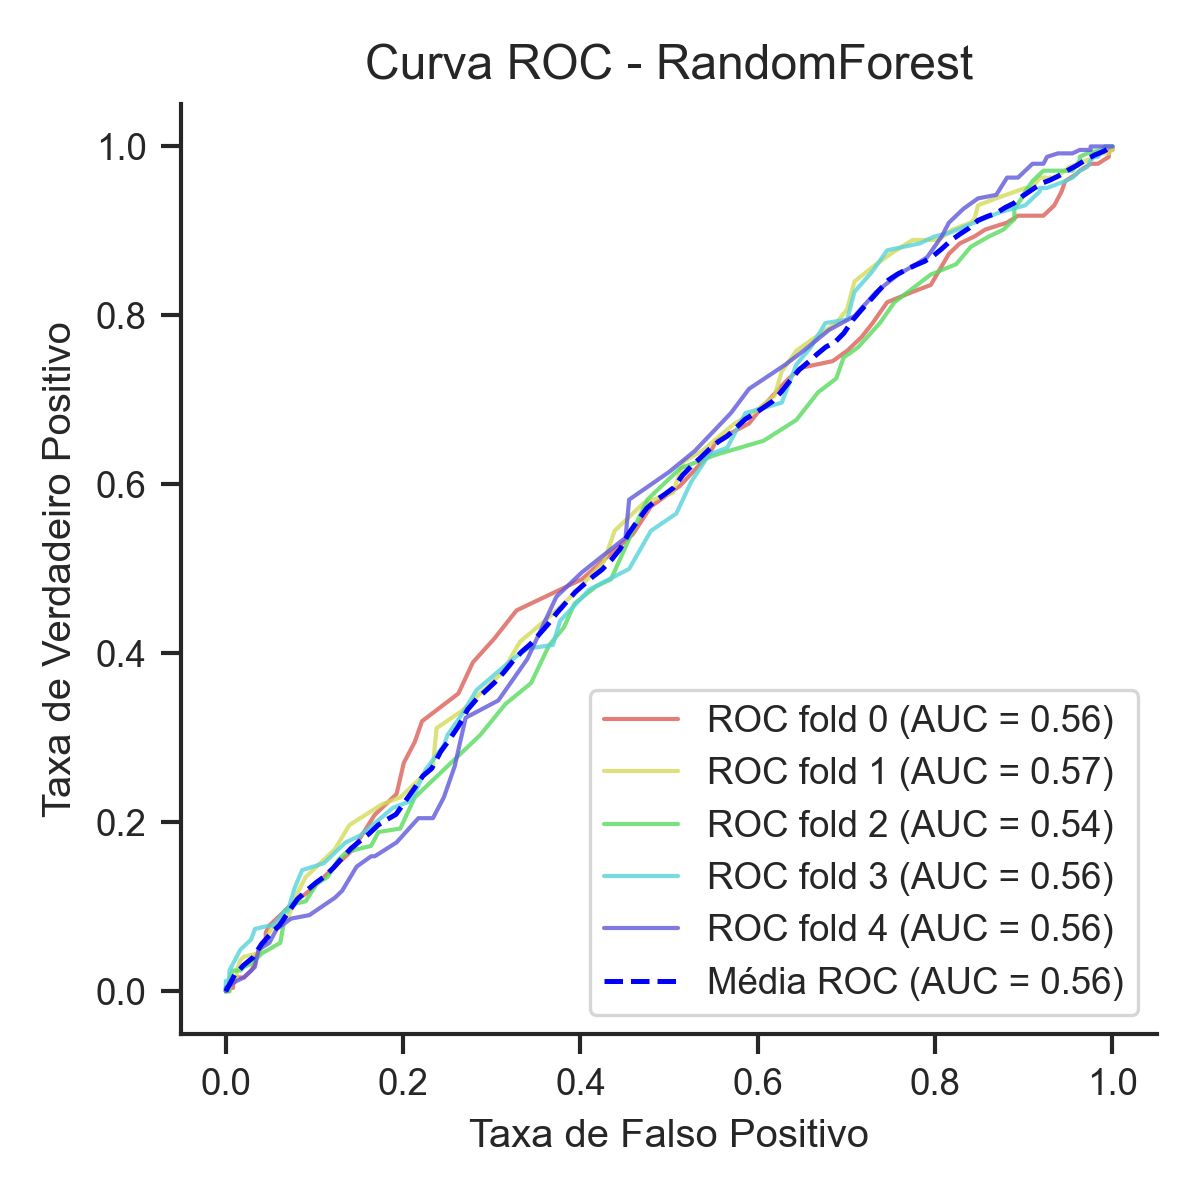
\includegraphics[width=\textwidth]{USPSC-img/Curva ROC - RandomForest.png}
	\end{minipage}
	\hfill
	\begin{minipage}[t]{0.28\textwidth}
		\centering
		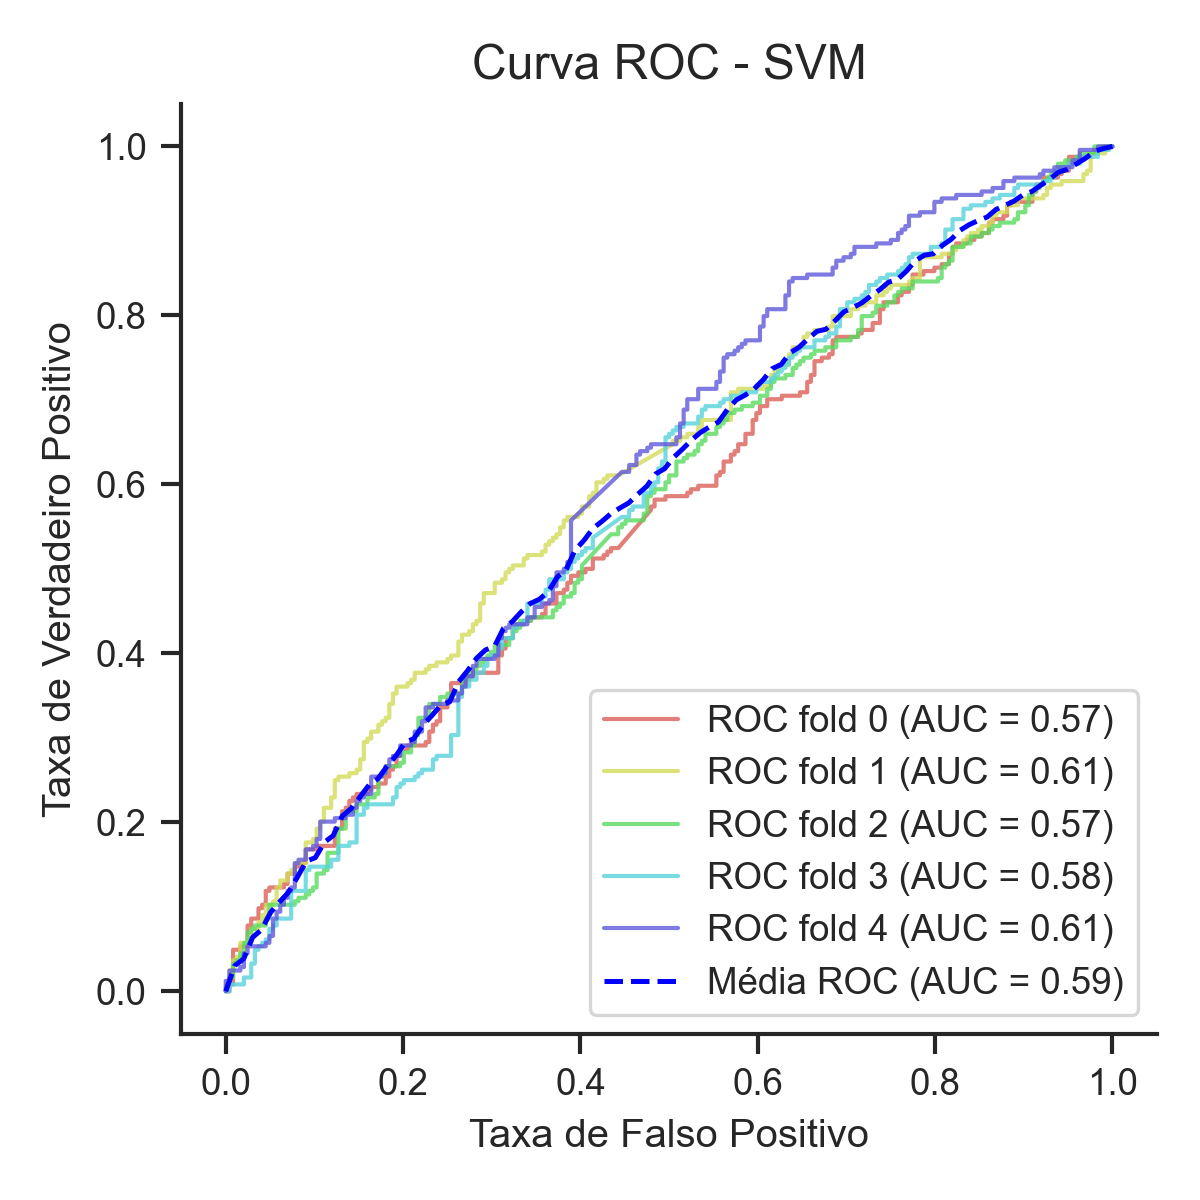
\includegraphics[width=\textwidth]{USPSC-img/Curva ROC - SVM.png}
	\end{minipage}
	\hfill
	\begin{minipage}[t]{0.28\textwidth}
		\centering
		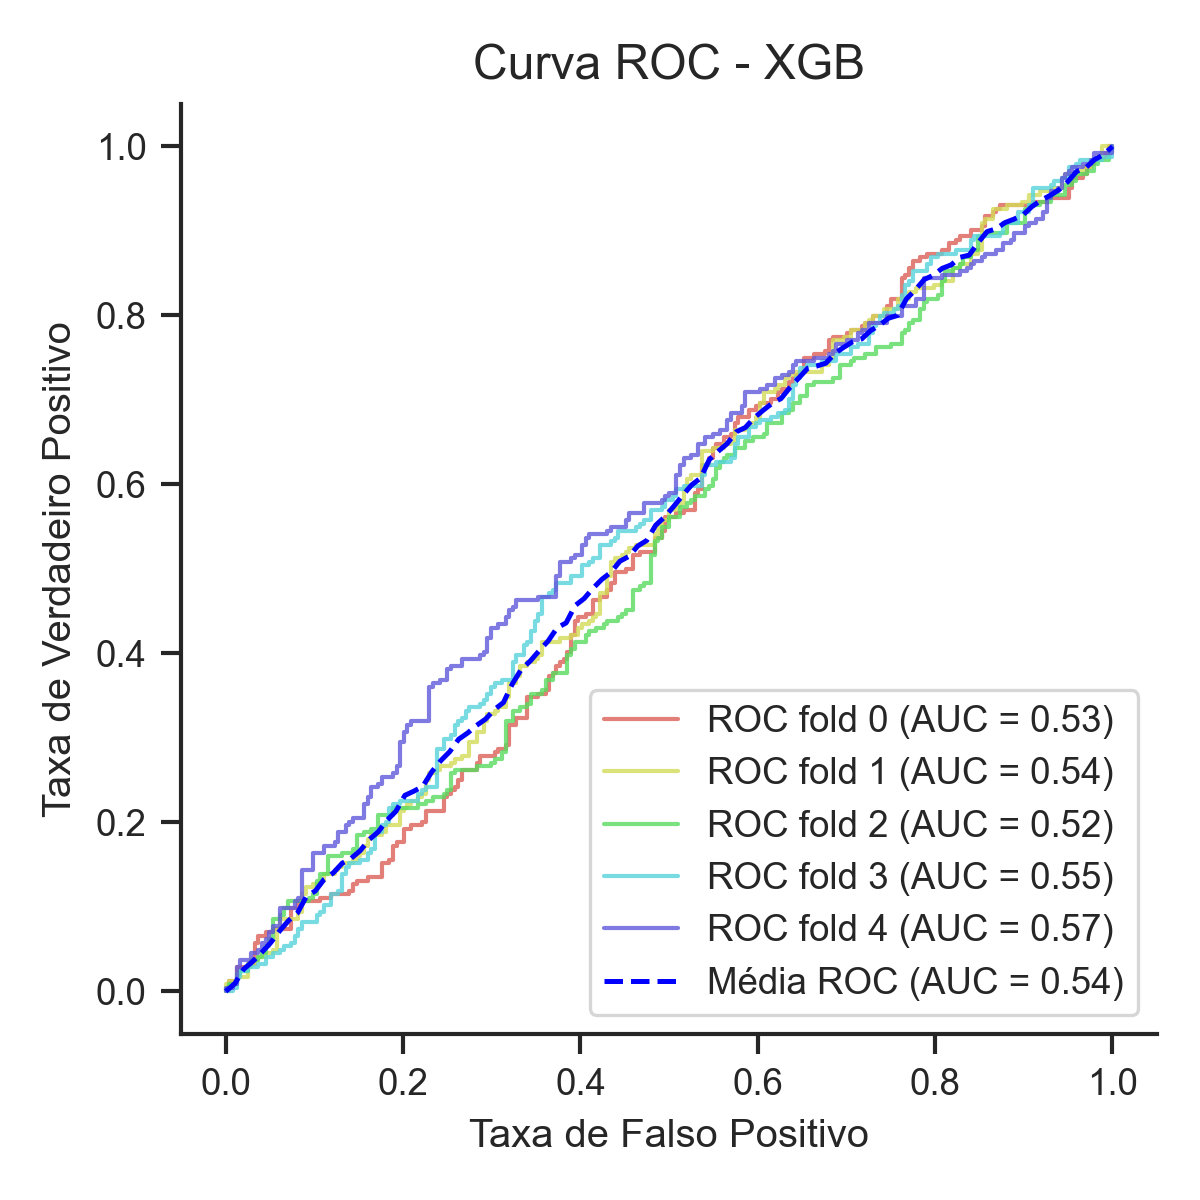
\includegraphics[width=\textwidth]{USPSC-img/Curva ROC - XGB.png}
	\end{minipage}
	
	\begin{center}
		Fonte: Autor (2023).
	\end{center}
\end{figure}

De acordo com as curvas ROC, é possível observar que nenhum dos modelos se destacou em relação aos outros no treinamento sem a otimização de hiperparâmetros. O classificador que obteve o melhor AUC durante o treinamento foi o SVM, com uma área no valor de 0.59.

Na \autoref{tab:treinoSemTunagem}, é apresentado um resumo dos resultados obtidos durante o treinamento e a análise revela \textit{insights} importantes sobre o desempenho dos modelos. Observando as métricas fornecidas, pode-se observar que o modelo SVM alcançou a maior acurácia, precisão e AUC entre todos os classificadores, indicando uma melhor capacidade geral de fazer previsões corretas e distinguir entre as classes positiva e negativa. Por outro lado, o modelo KNN demonstrou o desempenho mais baixo em todas essas métricas, sugerindo que sua capacidade preditiva pode ser menos confiável em comparação com os outros modelos.

\begin{table}[H]
	\IBGEtab{
		\caption{\centering\label{tab:treinoSemTunagem}Resultados obtidos após o treinamento dos modelos sem otimização de hiperparâmetros.}
	}
	{
		\begin{tabular}{lcccc}
			\toprule
			\textbf{Modelo} & \textbf{Acurácia} & \textbf{Precisão} & \textbf{Recall} & \textbf{AUC} \\
			\midrule \midrule
			GradientBoosting & 0.555738 & 0.555502 & 0.562295 & 0.581794 \\
			\midrule
			KNN & 0.525410 & 0.525395 & 0.519672 & 0.534181 \\
			\midrule
			LGBM & 0.539754 & 0.539814 & 0.533607 & 0.552842 \\
			\midrule
			LogisticRegression & 0.559426 & 0.559606 & 0.557377 & 0.585189 \\
			\midrule
			RandomForest & 0.534426 & 0.533356 & 0.550820 & 0.550509 \\
			\midrule
			SVM & 0.563115 & 0.563822 & 0.555738 & 0.586848 \\
			\midrule
			XGB & 0.534426 & 0.534750 & 0.527869 & 0.542001 \\
			\bottomrule
		\end{tabular}
	}
	{
		\fonte{\centering{Autor (2023).}}
	}
\end{table}

\subsubsection{Treinamento com otimização de hiperparâmetros}

A etapa subsequente do treinamento dos modelos envolveu a otimização de hiperparâmetros para melhorar o desempenho de cada classificador. Na \autoref{img:hiperparametros}, são apresentados quais conjuntos de hiperparâmetros foram considerados para cada um dos modelos testados. A estratégia visava encontrar a combinação ideal de hiperparâmetros que maximizasse o desempenho preditivo de cada modelo.

\begin{figure}[H]
	\centering
	\caption{\label{img:hiperparametros}Classificadores e seus respectivos conjuntos de hiperparâmetros testados na etapa de treinamento com otimização.}
	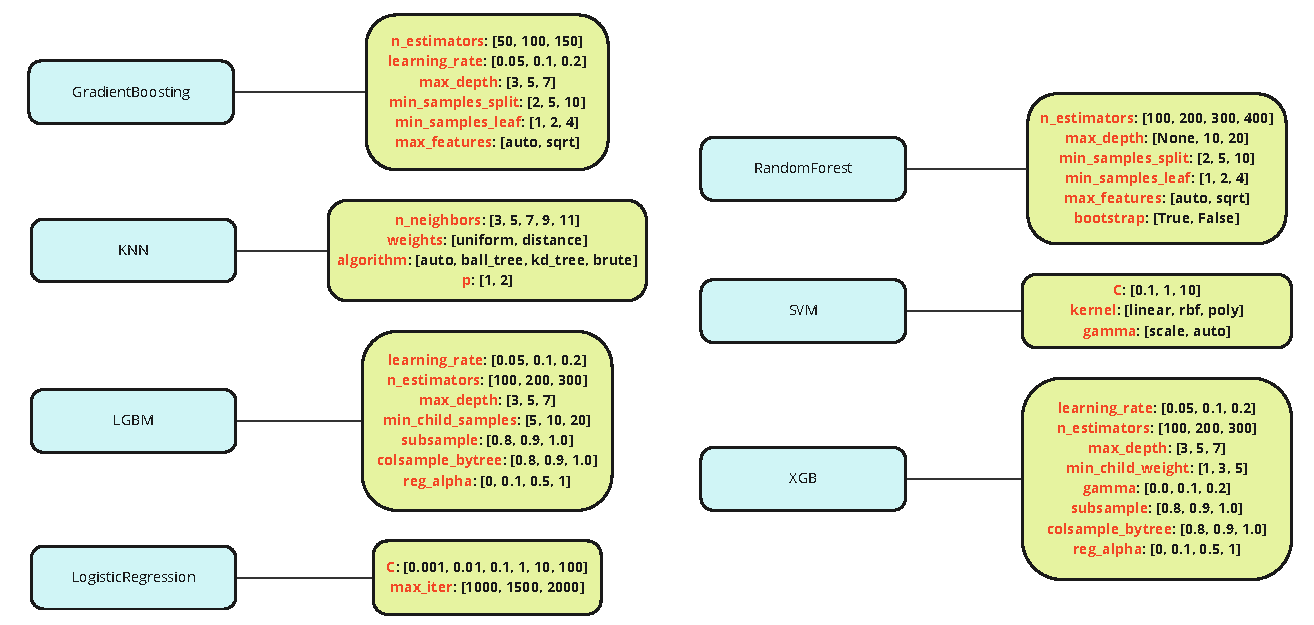
\includegraphics[scale=0.7]{USPSC-img/hiperparametros.pdf}
	\begin{center}
		Fonte: Autor (2023).
	\end{center}
\end{figure}

O treinamento desta etapa seguiu exatamente a mesma metodologia explicada na \autoref{sec:treinoSemHiperparametros}, com a única diferença sendo que, dentro do \textit{loop} que percorre cada modelo, o \textit{GridSearchCV} foi configurado para explorar o espaço de hiperparâmetros definido para cada classificador. O conjunto de hiperparâmetros que proporcionou o melhor desempenho, medido pela métrica da área sob a curva ROC, foi selecionado como a configuração ótima para aquele modelo específico. Cabe ressaltar essa foi a métrica escolhida como critério principal para a otimização de hiperparâmetros, uma vez que fornece uma medida robusta da capacidade discriminativa dos modelos.

Na \autoref{img:curvasRocComTunagem}, é apresentada uma comparação das curvas ROC de cada um dos modelos nos dois métodos de treinamento (com e sem otimização de hiperparâmetros). Nota-se que, no treinamento sem otimização, os classificadores GradientBoosting, LogisticRegression e SVM demonstram um desempenho superior em relação aos demais modelos, evidenciado pelo posicionamento dessas três curvas acima das demais. No entanto, no treinamento com otimização, percebe-se uma maior proximidade entre as curvas, indicando que os modelos conseguiram aprimorar o desempenho, mesmo que marginalmente, com a otimização.

\begin{figure}
	\centering
	\caption{\label{img:curvasRocComTunagem}Comparação das curvas ROC para cada classificador nas etapas de treinamento com e sem otimização de hiperparâmetros.}
	
	\begin{minipage}[t]{0.45\textwidth}
		\centering
		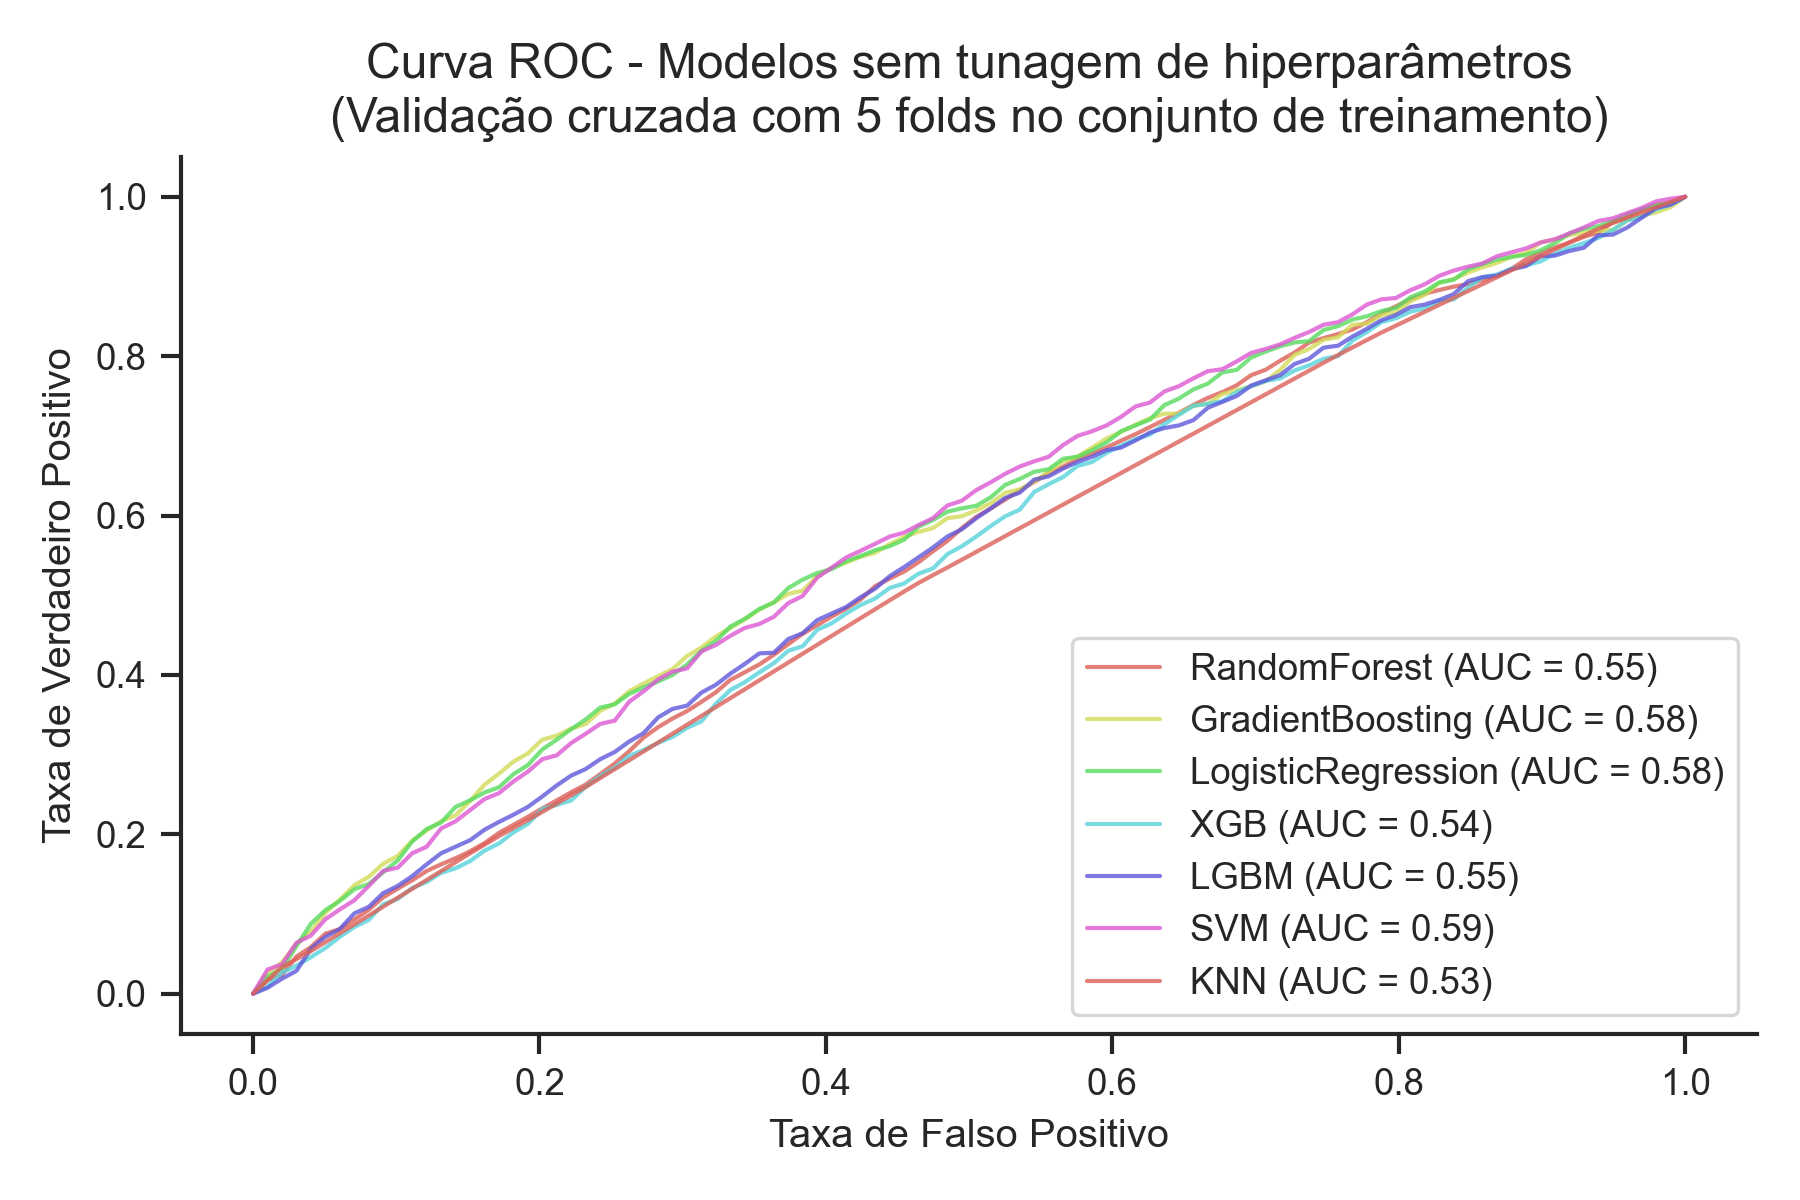
\includegraphics[width=\textwidth]{USPSC-img/curva_roc_modelos_sem_tunagem_hiperparametros.png}
	\end{minipage}
	\hfill
	\begin{minipage}[t]{0.45\textwidth}
		\centering
		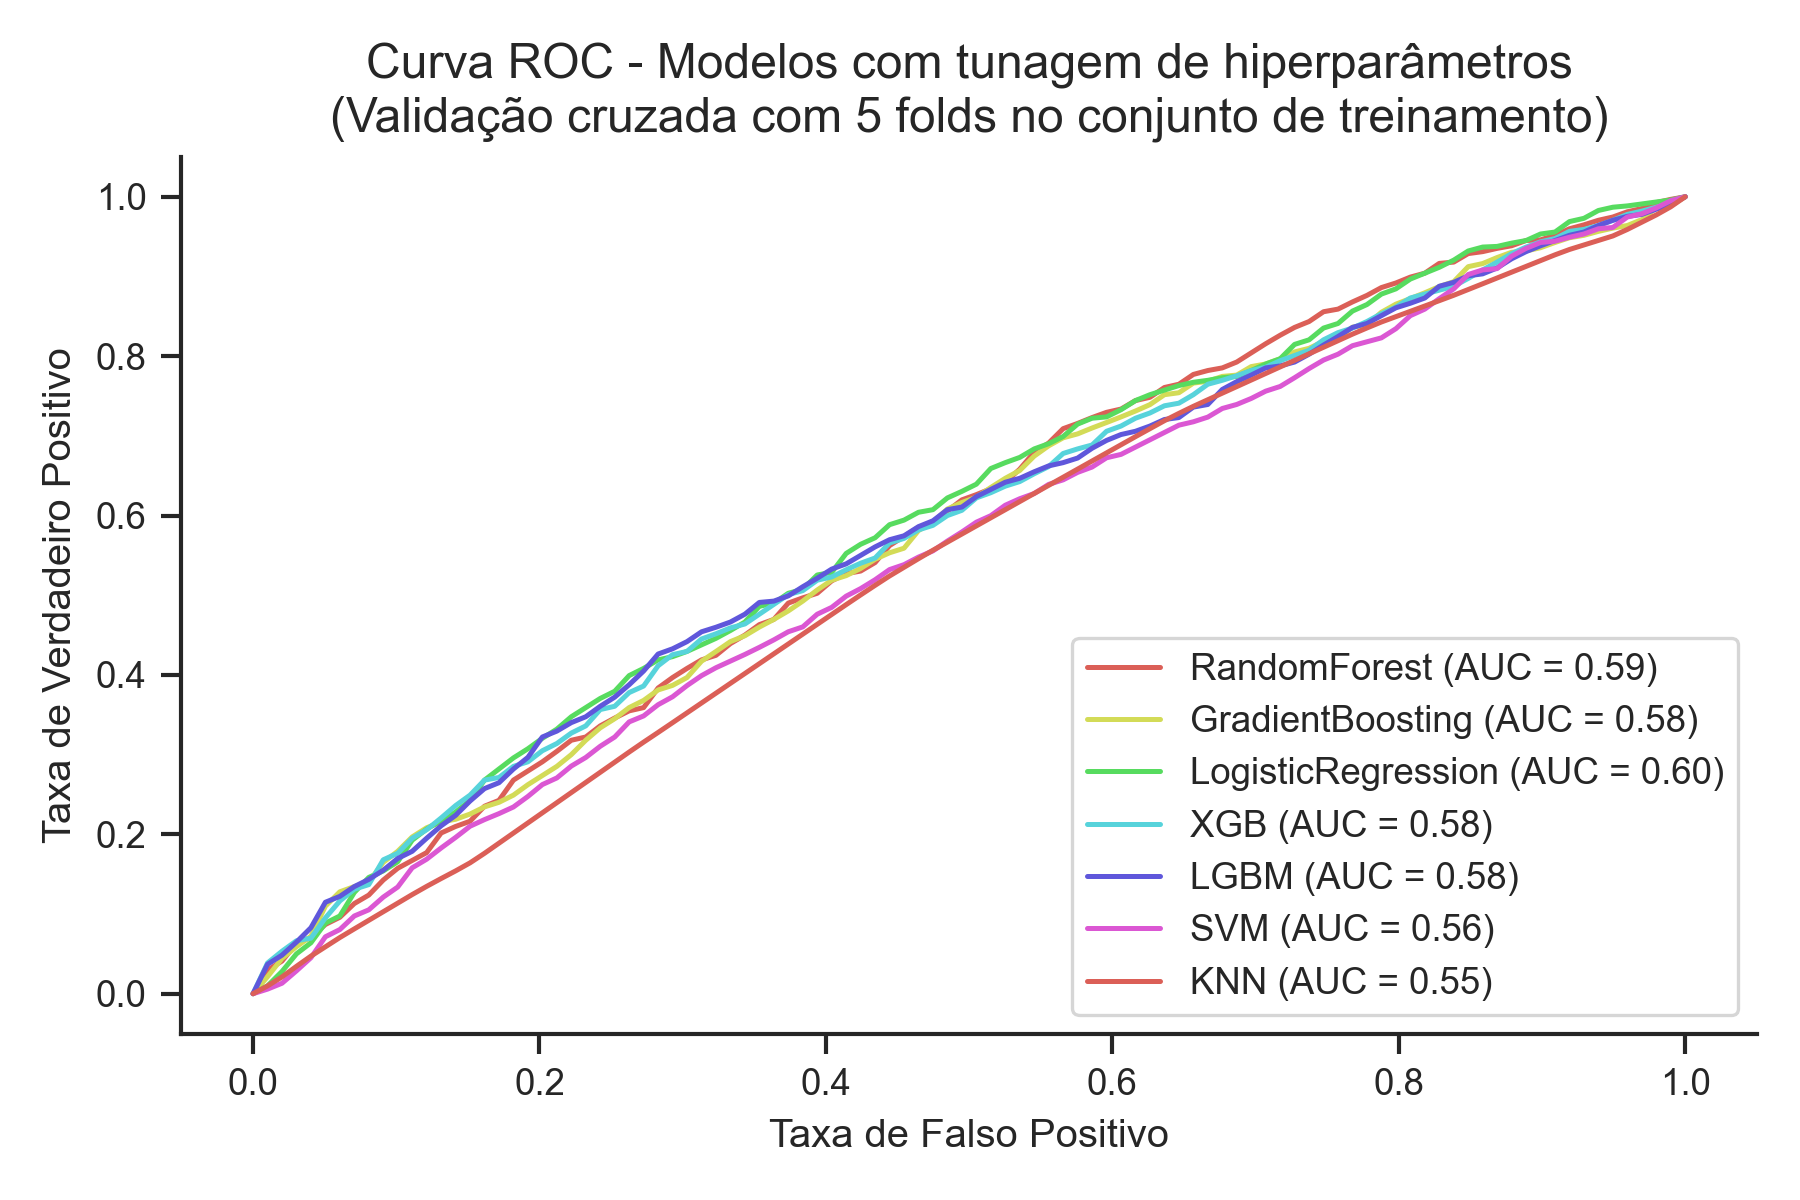
\includegraphics[width=\textwidth]{USPSC-img/curva_roc_modelos_com_tunagem_hiperparametros.png}
	\end{minipage}
	
	\begin{center}
		Fonte: Autor (2023).
	\end{center}
\end{figure}

Na \autoref{tab:treinoComTunagem}, são apresentados os resultados obtidos no treinamento com otimização. Observando os resultados, é possível destacar que o modelo LogisticRegression se sobressai em várias métricas, apresentando a mais alta acurácia, precisão e AUC entre todos os classificadores. Esse desempenho superior sugere que o modelo LogisticRegression é mais capaz de fazer previsões corretas e distinguir entre as classes positiva e negativa.

No entanto, é crucial considerar que o desempenho de um modelo pode variar dependendo do contexto específico e dos objetivos da aplicação. Por exemplo, se o foco principal for minimizar falsos negativos (identificar corretamente casos de reinternação), pode-se observar que o modelo SVM possui um recall notavelmente alto. Isso indica que o SVM é mais eficaz em capturar a totalidade das instâncias positivas em comparação com outros modelos. Dessa forma, a escolha do \q{melhor} modelo depende dos requisitos específicos do problema em questão. O LogisticRegression destaca-se em termos gerais, enquanto o SVM parece ter uma capacidade superior em identificar casos de reinternação.

\begin{table}
	\IBGEtab{
		\caption{\centering\label{tab:treinoComTunagem}Resultados obtidos após o treinamento dos modelos com otimização de hiperparâmetros.}
	}
	{
		\begin{tabular}{lcccc}
			\toprule
			\textbf{Modelo} & \textbf{Acurácia} & \textbf{Precisão} & \textbf{Recall} & \textbf{AUC} \\
			\midrule \midrule
			RandomForest & 0.554917 & 0.552547 & 0.577719 & 0.579562 \\
			\midrule
			GradientBoosting & 0.550615 & 0.550843 & 0.549116 & 0.571107 \\
			\midrule
			LogisticRegression & 0.564208 & 0.564933 & 0.559426 & 0.587308 \\
			\midrule
			XGB & 0.544608 & 0.544739 & 0.541992 & 0.560123 \\
			\midrule
			LGBM & 0.543404 & 0.543352 & 0.543370 & 0.558586 \\
			\midrule
			SVM & 0.547154 & 0.543553 & 0.663115 & 0.581624 \\
			\midrule
			KNN & 0.528811 & 0.528966 & 0.524836 & 0.537458 \\
			\bottomrule
		\end{tabular}
	}
	{
		\fonte{\centering{Autor (2023).}}
	}
\end{table}

\subsubsection{Validação no conjunto de teste}

A fase de validação dos modelos, agora equipados com os melhores conjuntos de hiperparâmetros, representa um passo importante para avaliar a capacidade preditiva no mundo real. Na \autoref{img:curvaRocTeste}, são exibidas as curvas ROC de cada modelo, revelando que os classificadores XGB e LGBM destacaram-se pela capacidade de generalização. Esta capacidade demonstra a habilidade desses modelos em prever com maior precisão instâncias que não foram previamente observadas durante o treinamento.

\begin{figure}[H]
	\centering
	\caption{\label{img:curvaRocTeste}Curvas ROC para cada classificador na etapa de validação no conjunto de teste.}
	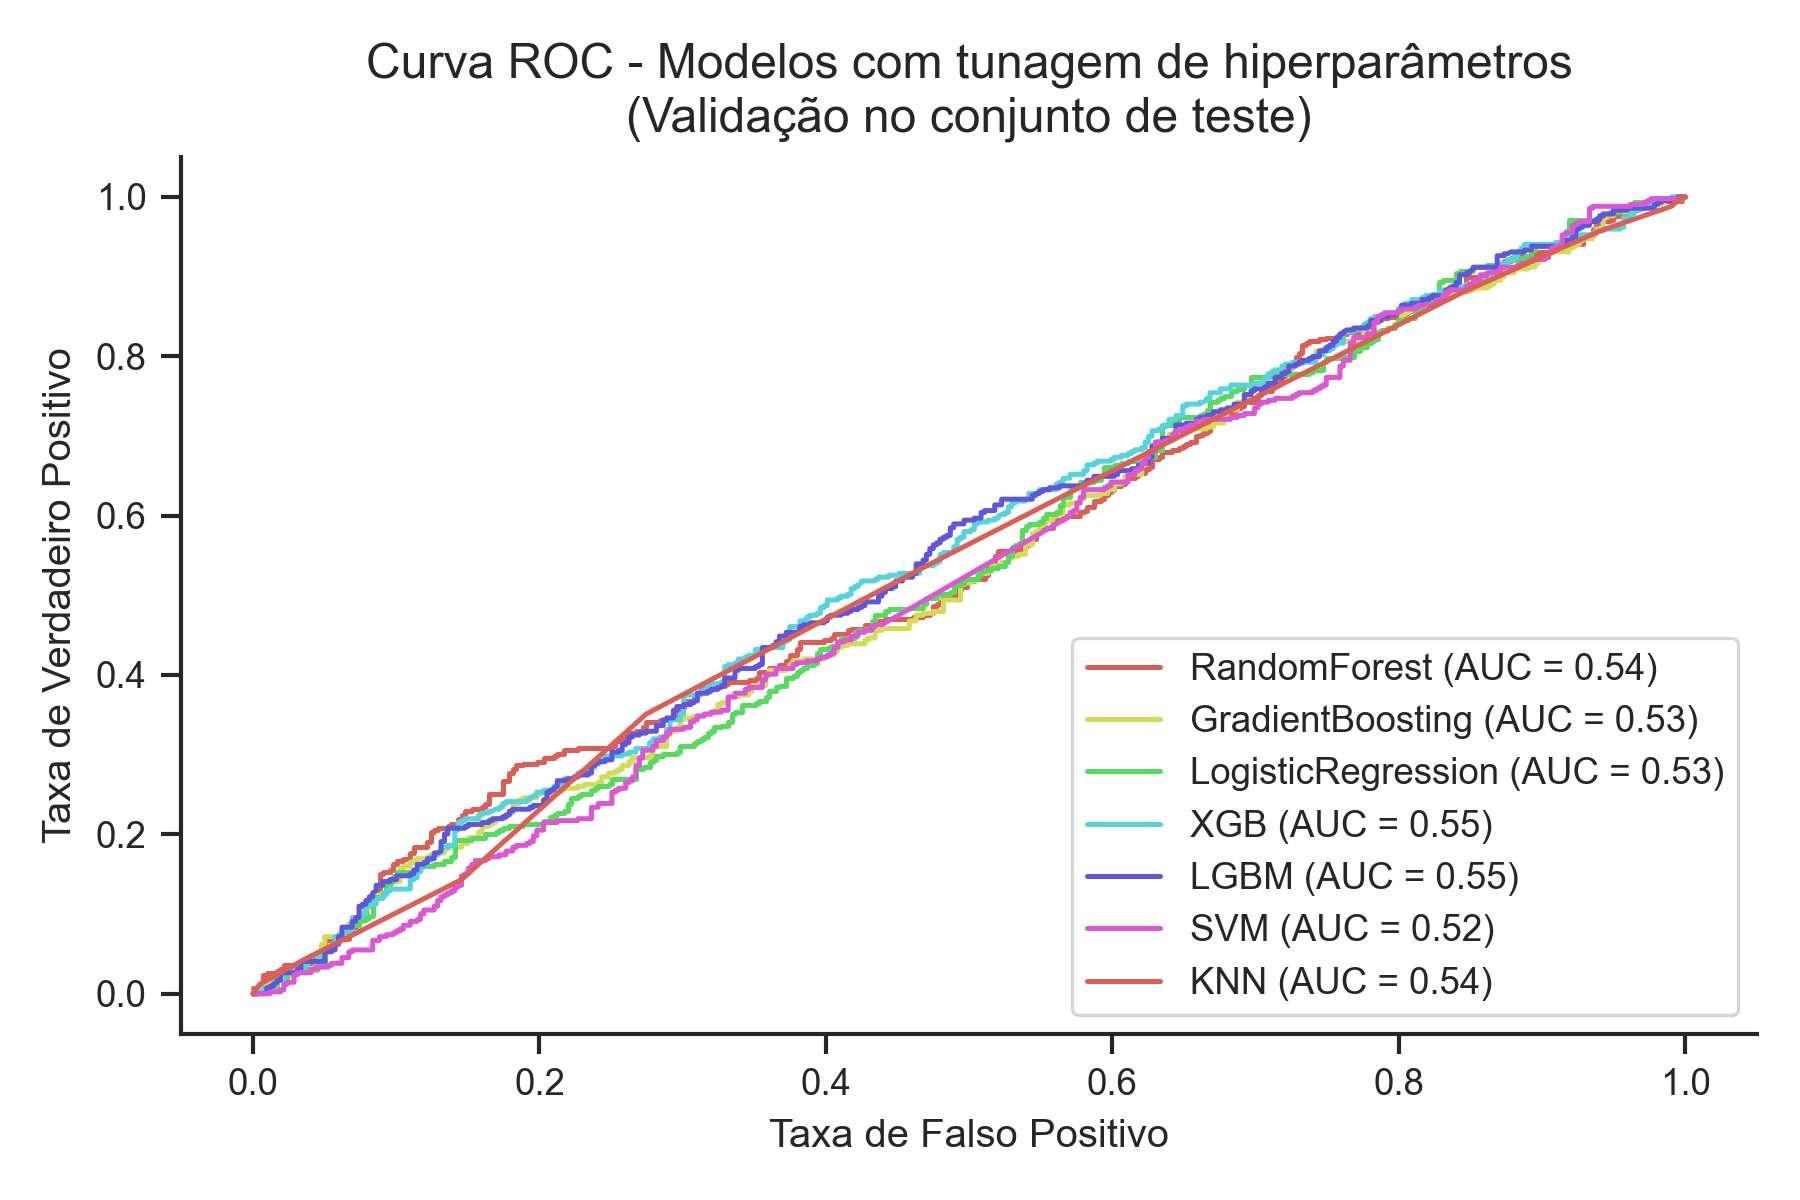
\includegraphics[scale=0.7]{USPSC-img/curva_roc_modelos_teste.png}
	\begin{center}
		Fonte: Autor (2023).
	\end{center}
\end{figure}

Na \autoref{tab:validacaoTeste}, são apresentados os resultados da validação no conjunto de teste, fornecendo uma análise abrangente das métricas-chave. Notavelmente, o modelo LGBM liderou em acurácia e precisão, enquanto o XGB liderou em AUC, mesmo que a discrepância entre as métricas de ambos os classificadores esteja na ordem da terceira casa decimal. O modelo SVM se destaca, novamente, exibindo um valor notavelmente alto de \textit{recall}.

\begin{table}
	\IBGEtab{
		\caption{\centering\label{tab:validacaoTeste}Resultados obtidos na validação no conjunto de teste.}
	}
	{
		\begin{tabular}{lcccc}
			\toprule
			\textbf{Modelo} & \textbf{Acurácia} & \textbf{Precisão} & \textbf{Recall} & \textbf{AUC} \\
			\midrule \midrule
			RandomForest & 0.510740 & 0.509890 & 0.553699 & 0.541202 \\
			\midrule
			GradientBoosting & 0.522673 & 0.521542 & 0.548926 & 0.545679 \\
			\midrule
			LogisticRegression & 0.509547 & 0.509569 & 0.508353 & 0.532521 \\
			\midrule
			XGB & 0.532220 & 0.531915 & 0.536993 & 0.554218 \\
			\midrule
			LGBM & 0.533413 & 0.533654 & 0.529833 & 0.551911 \\
			\midrule
			SVM & 0.522673 & 0.518591 & 0.632458 & 0.520830 \\
			\midrule
			KNN & 0.533413 & 0.533333 & 0.534606 & 0.541322 \\
			\bottomrule
		\end{tabular}
	}
	{
		\fonte{\centering{Autor (2023).}}
	}
\end{table}

Na \autoref{img:comparacaoMetricas}, é apresentado um resumo abrangente, comparando todas as métricas em todas as fases de validação, incluindo treinamento sem e com otimização, bem como no conjunto de teste, para todos os modelos.

\begin{figure}
	\centering
	\caption{\label{img:comparacaoMetricas}Comparação das métricas de desempenho em diferentes etapas de validação (treinamento sem e com otimização, e teste) para os modelos.}
	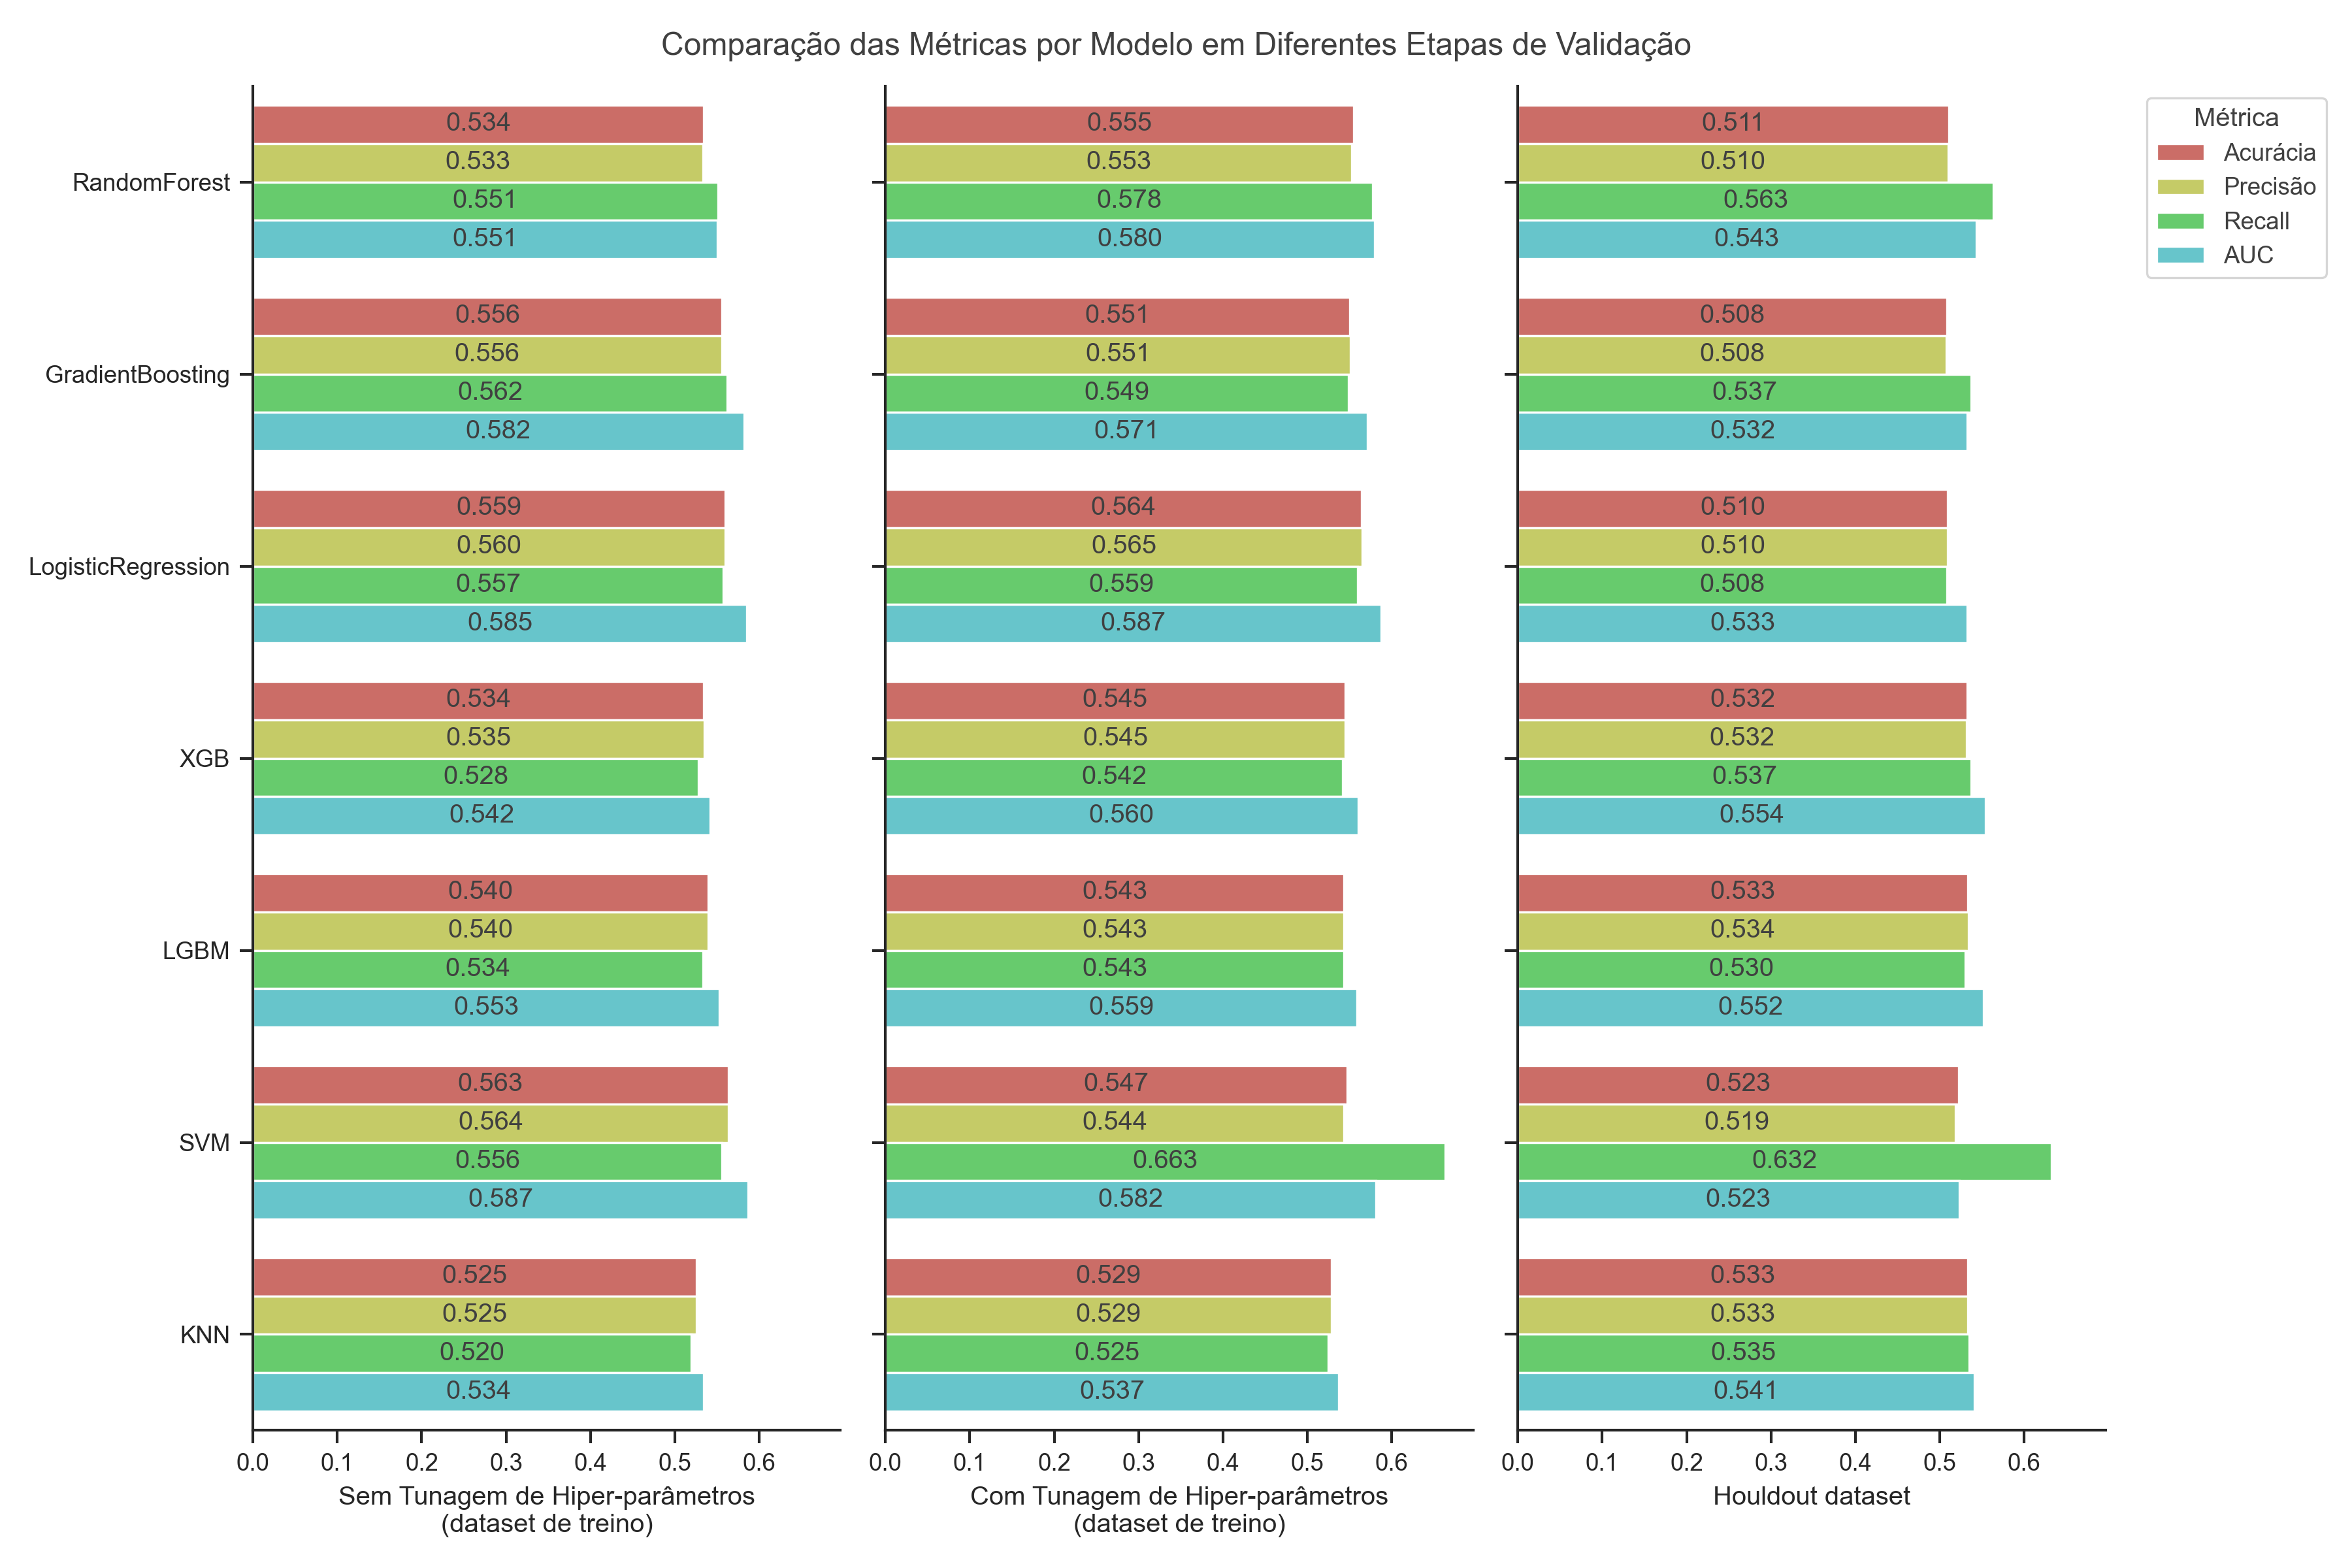
\includegraphics[scale=0.5]{USPSC-img/comparacao_metricas_por_modelo.png}
	\begin{center}
		Fonte: Autor (2023).
	\end{center}
\end{figure}

Também é possível observar, na \autoref{img:variacaoMetricas}, a variação percentual das métricas no conjunto de teste em comparação com as métricas na etapa de otimização. Com exceção do classificador KNN, todos os modelos apresentaram uma degradação nas métricas. Notavelmente, o LogisticRegression foi o modelo com a pior capacidade de generalização, registrando uma variação de aproximadamente -8\% em todas as métricas. Em contrapartida, os modelos XGB e LGBM sofreram as menores quedas, mantendo-se próximos do valor de -4\%. Considerando esses resultados, ambos os classificadores se destacam como candidatos viáveis para a escolha do melhor modelo. Optou-se por selecionar o modelo LGBM, que será utilizado na análise subsequente das variáveis mais importantes, empregando a abordagem SHAP.

\begin{figure}
	\centering
	\caption{\label{img:variacaoMetricas}Variação percentual das métricas no conjunto de teste em comparação com as métricas na etapa de otimização.}
	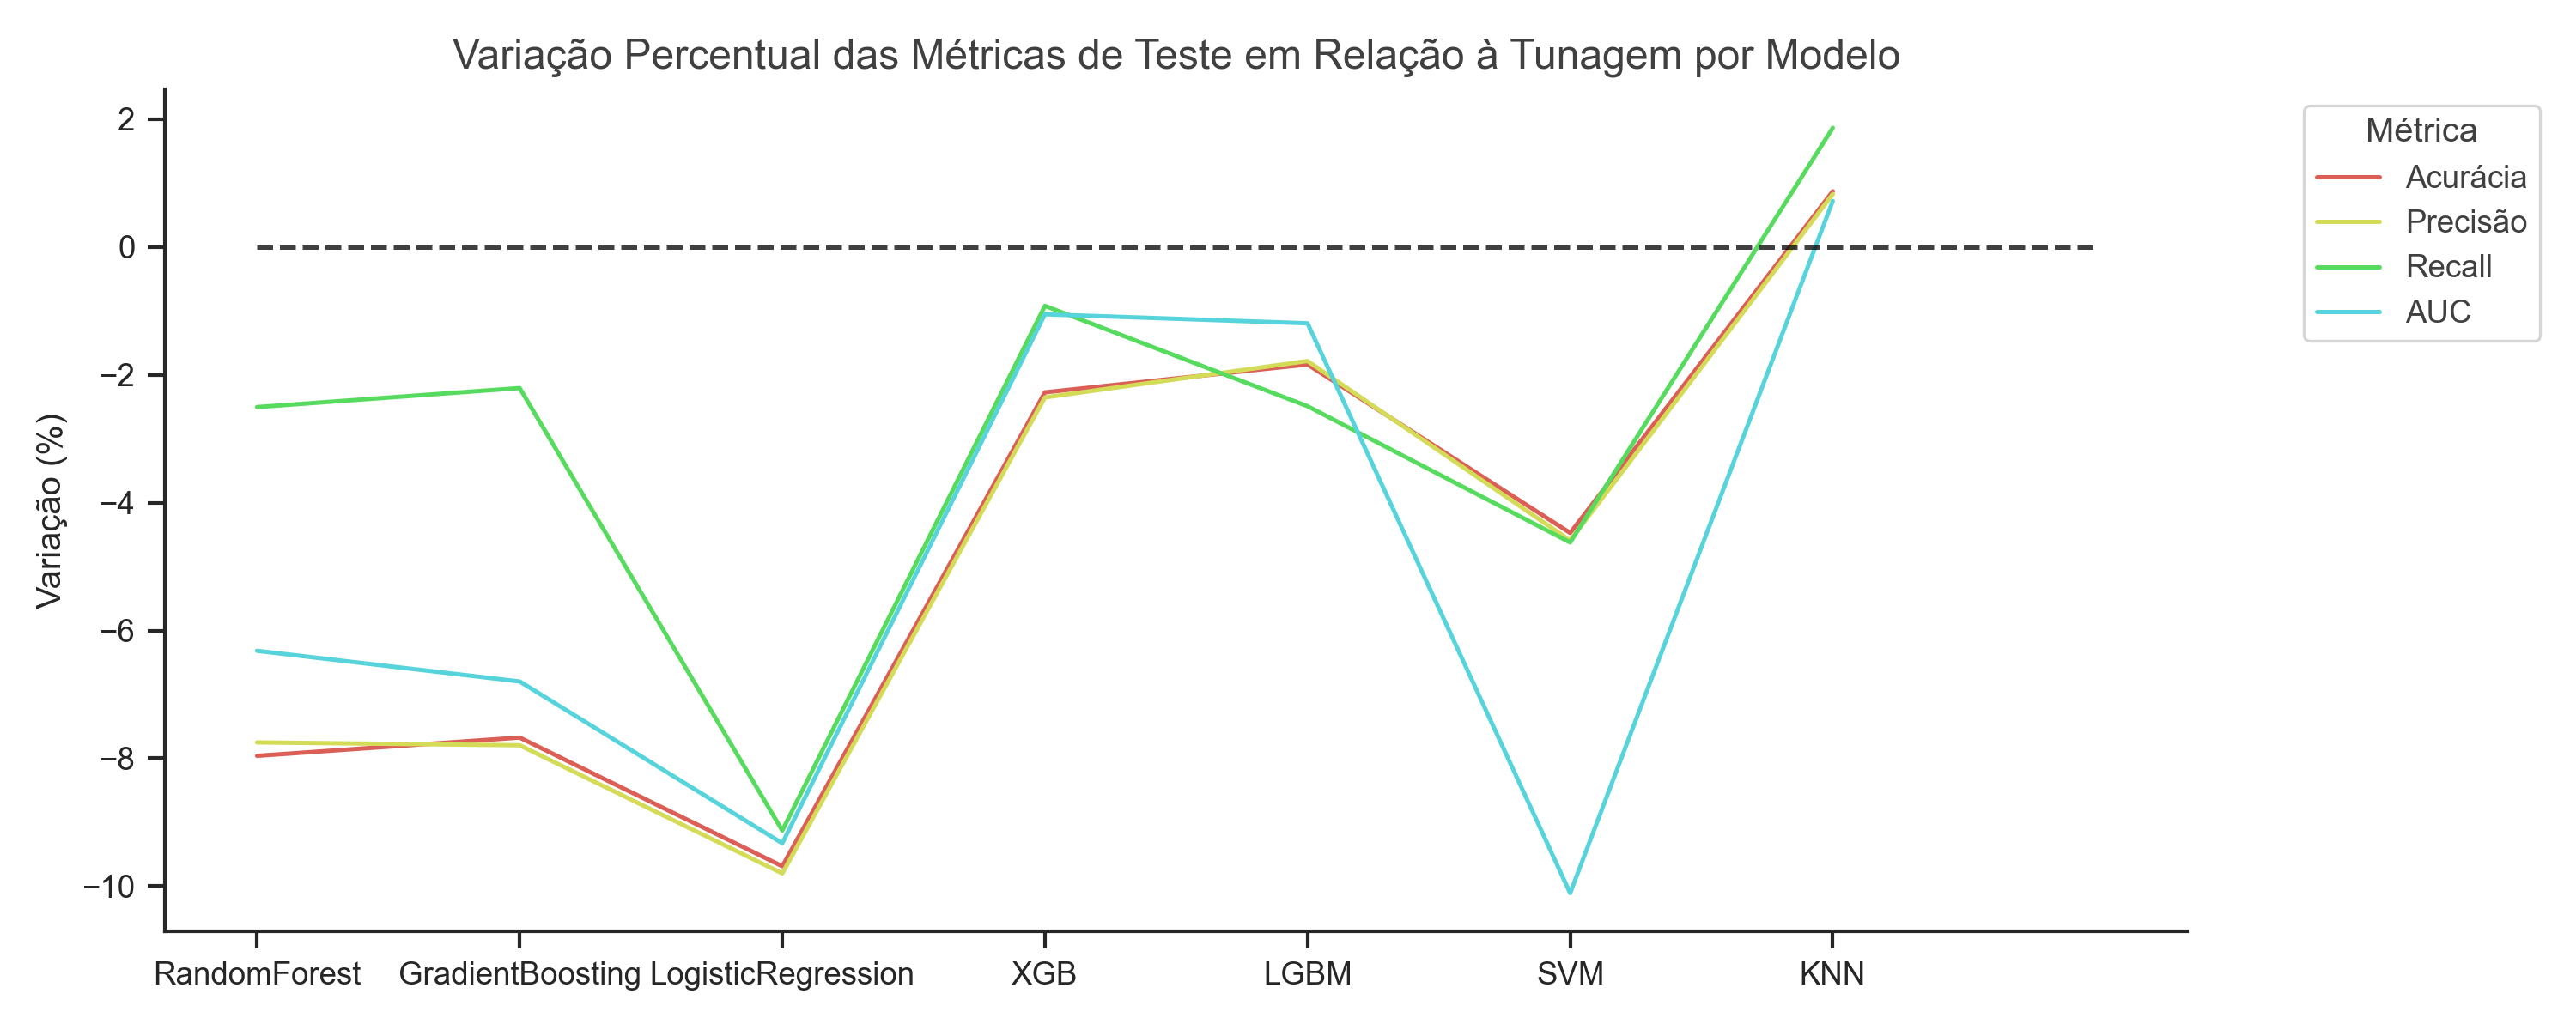
\includegraphics[scale=0.7]{USPSC-img/variacao_pct_metricas_teste_por_modelo.png}
	\begin{center}
		Fonte: Autor (2023).
	\end{center}
\end{figure}

\subsection{Análise de variáveis mais importantes}

Esta seção aborda a análise das variáveis mais importantes para as predições do modelo, empregando o método SHAP. A escolha desse método de explicação é respaldada pelas vantagens detalhadas na \autoref{sec:shap}, onde se destaca sua capacidade de atribuir valores a cada variável (chamados de valores SHAP), oferecendo uma interpretação mais granular e confiável do impacto de cada variável nas predições do modelo \cite{Shap2017}.

A biblioteca SHAP possui diversas ferramentas úteis para análise da importância de variáveis em modelos de aprendizado de máquina. Entre as funcionalidades notáveis estão a capacidade de gerar gráficos claros e informativos, como o gráfico \textit{beeswarm}. Esse gráfico foi projetado para exibir um resumo denso de informações de como as principais variáveis em um conjunto de dados impactam a saída do modelo. Na \autoref{img:exemploBeeswarm}, é exibido um exemplo de um gráfico \textit{beeswarm} de um modelo treinado com o conjunto de dados \textit{UCI adult income dataset} (conjunto de dados de renda adulta da UCI, em tradução livre), que é usado em tarefas de classificação para prever se pessoas granharam mais de 50 mil dólares durante os anos 90.

\begin{figure}
	\centering
	\caption{\label{img:exemploBeeswarm}Exemplo de gráfico \textit{beeswarm} para classificador treinado com o \textit{UCI adult income dataset}.}
	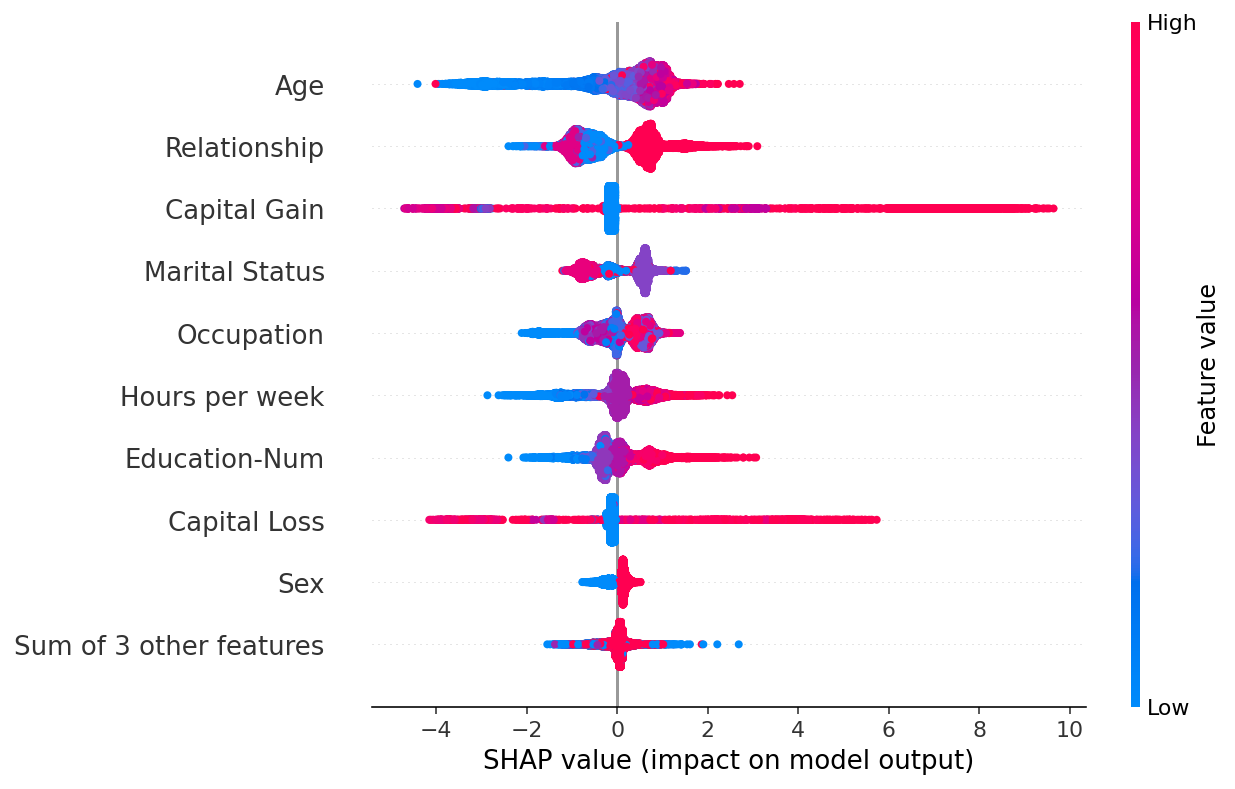
\includegraphics[scale=0.7]{USPSC-img/exemplo_beeswarm.png}
	\begin{center}
		Fonte: Autor (2023).
	\end{center}
\end{figure}

Cada instância da explicação dada é representada por um único ponto em cada linha de variável. A posição $x$ do ponto é determinada pelo valor SHAP dessa variável, e os pontos \q{se acumulam} ao longo de cada linha de variável para mostrar a densidade. A cor é usada para exibir o valor original de uma variável. No exemplo da \autoref{img:exemploBeeswarm} pode-se notar que a idade é a característica mais importante em média, e que os jovens (azuis) têm menos probabilidade de ganhar mais de 50 mil.

A análise da importância das variáveis neste trabalho foi conduzida utilizando essa mesma ferramenta (\textit{beeswarm}). O propósito central desta análise é proporcionar insights acionáveis para a prática clínica e estratégias de intervenção. A identificação das variáveis mais significativas não apenas informa sobre os fatores críticos associados às reinternações, mas também orienta a implementação de intervenções preventivas específicas. A partir dessas informações, estratégias personalizadas podem ser desenvolvidas, desde ajustes individuais no tratamento até a criação de campanhas sazonais direcionadas a grupos específicos de pacientes. Na \autoref{img:topFeatures}, é apresentado o \textit{ranking} com as 15 variáveis mais importantes para o output do modelo LGBM.

\begin{figure}
	\centering
	\caption{\label{img:topFeatures}Gráfico \textit{beeswarm} com as 15 variáveis mais importantes para classificador LGBM.}
	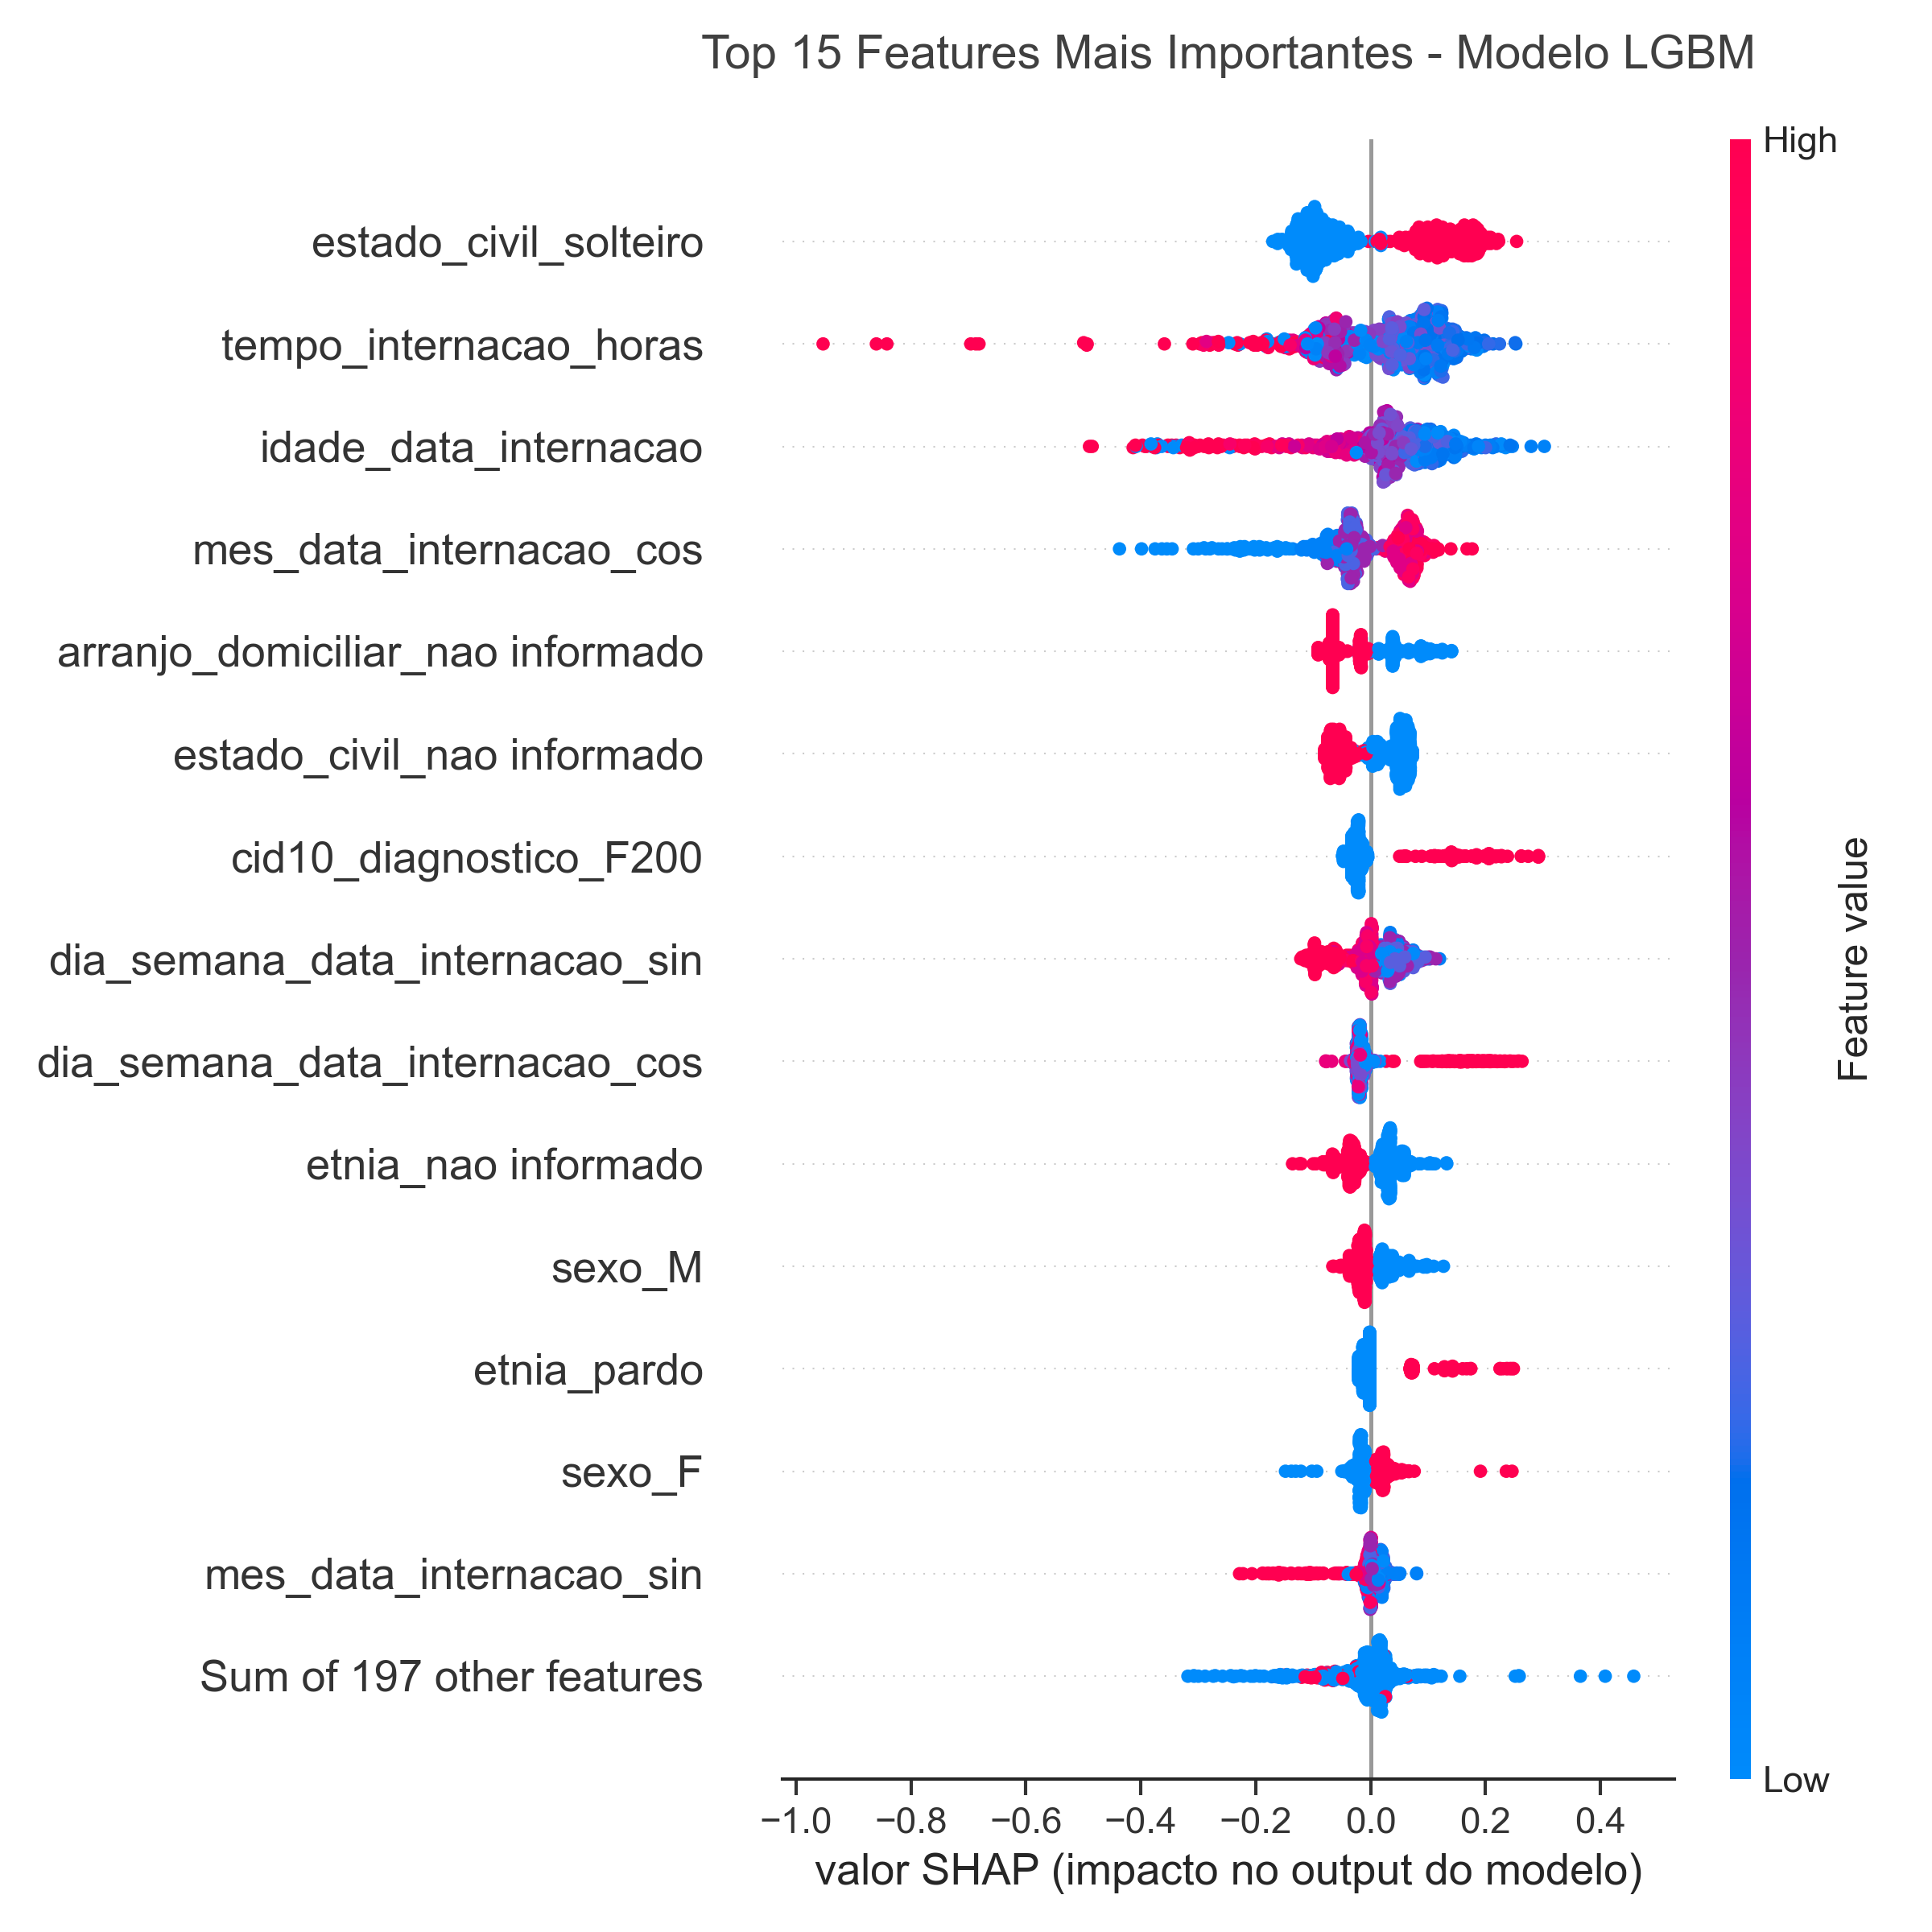
\includegraphics[scale=0.7]{USPSC-img/top-features-lgbm.png}
	\begin{center}
		Fonte: Autor (2023).
	\end{center}
\end{figure}

A análise da \autoref{img:topFeatures} traz \textit{insights} cruciais sobre as variáveis mais impactantes no contexto da previsão de reinternações hospitalares. A variável que se destacou como a mais importante foi \q{\textbf{estado\_civil\_solteiro}}, que assume valores binários 0 e 1. Quando esta variável assume o valor 1, indicando que o paciente é solteiro, observou-se uma correlação significativa com uma maior probabilidade de reinternação.

Duas variáveis relacionadas à temporalidade se mostraram igualmente essenciais. A \q{\textbf{tempo\_internacao\_horas}} emergiu como a segunda variável mais importante, indicando que tempos mais curtos de internação estão associados a uma maior probabilidade de reinternação. Similarmente, a \q{\textbf{idade\_data\_internacao}} ocupou a terceira posição no \textit{ranking}, destacando que pacientes mais jovens, identificados pela coloração azul no gráfico, apresentam uma maior propensão à reinternação.

A análise também abordou variáveis que passaram por transformações trigonométricas, como \q{\textbf{mes\_data\_internacao}} e \q{\textbf{dia\_semana\_data\_internacao}}. A presença dessas variáveis no \textit{ranking} sugere que padrões sazonais podem desempenhar um papel significativo na probabilidade de reinternação, fornecendo uma perspectiva valiosa para a implementação de estratégias preventivas.

Além disso, um destaque notável foi a variável representada pelo código F200 da lista CID-10 (Classificação Internacional de Doenças e Problemas Relacionados à Saúde), correspondente à esquizofrenia paranóide. Esta variável emergiu como uma indicação importante, sugerindo que pacientes admitidos com esse diagnóstico específico têm uma probabilidade substancialmente maior de reinternação.

Também é possível observar variáveis com o sufixo \q{não informado} entre as mais importantes. Esse sufixo indica que, para uma determinada instância do conjunto de dados, uma dada variável não foi preenchida no momento da admissão, ou foi preenchida exatamente com o status \q{não informado}. A presença de variáveis desse tipo no \textit{ranking} sugere que essa categoria tem uma influência discernível nas predições do modelo, indicando que a ausência de informações é um fator relevante para o entendimento do modelo sobre a probabilidade de reinternação. Contudo, essa interpretação deve ser feita com cautela, uma vez que\q{não informado} pode não representar uma característica intrínseca do paciente, mas sim uma lacuna nos registros.